%Jak dělat reference:
% \cite{baker}

%Jak dělat poznámky:
% \footnote{tralala}

% TO DO
% Některá vysvětlení rovnic mohou být málo srozumitelná, chtělo by to víc se rozepsat (hlavně při úrovni pana grafa (který podle mě je fyzik mezi porotci))
% přidat pod rovnice popis proměných
% ohybani svetla vysvetlit, prepocitavani namerenych spektro hodnot taky, jeste absolute humidity

%
\documentclass{cfp}  

%
\usepackage[utf8]{inputenc}
\usepackage{chngcntr}
% \usepackage[margin=1in,includeheadfoot,headheight=13.6pt,footskip=2cm]{geometry}
\usepackage{amsmath}
\usepackage{pgfplots}
\usepackage{listingsutf8}
\usepackage{graphicx}
\usepackage{amsfonts}
\usepackage{txfonts}
\usepackage[colorlinks=true,urlcolor=blue]{hyperref}
\usepackage{eurosym}
\usepackage{chemfig}
\usepackage[version=4]{mhchem}
\usepackage{multicol}
\usepackage[symbol*]{footmisc}
\usepackage{indentfirst}
\usepackage{mathtools}
\usepackage{fixltx2e}
\usepackage{siunitx}
% \usepackage{titlesec}
% \usepackage{float}
% \usepackage{fancyhdr}
% \usepackage{array}
% \usepackage{longtable}
% \usepackage{dirtytalk}
\pdfminorversion=5 
\pdfcompresslevel=9
\pdfobjcompresslevel=2

\counterwithin{figure}{section}
\counterwithin{equation}{section}
\renewcommand{\thefootnote}{\fnsymbol{footnote}}
\setlength{\parindent}{3ex}
\setlength{\parskip}{0ex}
\newcommand{\rpm}{\sbox0{$1$}\sbox2{$\scriptstyle\pm$}
  \raise\dimexpr(\ht0-\ht2)/2\relax\box2 }
\newcommand{\degree}{^{\circ}}
\begin{document} 


   \title{CFP-18-Hatalom}

   \subtitle{ Simulation of finding life and life supporting conditions on exoplanets }

   \author{J. Suchánek
   		  \inst{1}
		  \and          
          P. Novotný
   		  \inst{2}
   		  \and
   		  J. Janoušek
   		  \inst{3}
   		  \and
   		  Lukáš Völfl
   		  \inst{4}
   		  \and
   		  Martin Vítek
   		  \inst{5}
   		  \and
   		  Jakub Zeman
   		  \inst{6}
          }
          
   \institute{Gymnázium Opatov, Czech Republic\\
              \email{suchanek989@seznam.cz}
         \and
             Gymnázium Opatov, Czech Republic\\
             \email{patrik.novotny.jes@seznam.cz}
         \and
             Gymnázium Opatov, Czech Republic\\
             \email{honza.janousek.11@gmail.com}
         \and
             Gymnázium Opatov, Czech Republic\\
             \email{luky.volfl@gmail.com}
         \and
             Gymnázium Opatov, Czech Republic\\
             \email{martulavitek@seznam.cz}
         \and
             Gymnázium Opatov, Czech Republic\\
             \email{kubazeman@volny.cz}
             }

   \date{July 15, 2018}

% \abstract{}{}{}{}{}
 
  \abstract
  % context heading (optional)
  % {} leave it empty if necessary  
   {Our analysis, like our mission, deals with the detection of life and the conditions necessary for its creation and development.}
  % aims heading (mandatory)
   {This work aims to introduce the analysis of the data we made after the flight of our Cansat and partly our entire project.}
  % methods heading (mandatory)
   {We conducted two types of analysis, biological analysis, and calculations of other variables using our own models that we developed. These are approximation models that are all available on our Git. This document also serves as their documentation.}
  % results heading (mandatory)
   {Tested planet seems habitable and even contains both microscopic and macroscopic life identical in basic structure to the life on Earth.}
  % conclusions heading (optional), leave it empty if necessary 
   {The analysis was thorough enough to declare with near certainty that it is habitable for humans. The project has had some failures but the analysis has turned out correct.}

   \keywords{Cansat, Gram's staining, Greenhouse effect, Exoplanet properties, Kepler 62, Atmospheric spectroscopy}

   \maketitle
%
%________________________________________________________________

\section{Introduction}
\par Our vision of Cansat was to build an interplanetary probe, which should not take care of the process of getting to a planet but the landing. We are landing at another planet. The one we selected is a planet orbiting around star named Kepler 62. It cannot be seen by an eye from Earth and its radius is smaller than radius of our Sun. Kepler 62 is situated in Lyra constellation and it is nearly 1,200 light years away from the Solar System. There are 5 planets orbiting around Kepler 62. Two of them, “e” and “f”, are very interesting for us as they lay in the habitable zone.
\par Planet “e” lies on the inner side of the habitable zone. According to calculations made using its semi-major axis, it is too hot for the possibility of existence of life similarly to Venus. However, its sibling Kepler 62f is much more promising. We do not have every piece of data, but we know that in the given orbital distance from the Kepler 62, the planet should have temperature of -40$^\circ$C. However, if it had 5 times thicker atmosphere composed of CO\textsubscript{2}, which is not anything uncommon, liquid water could be present on the surface of the planet. Kepler 62 is a stable star with low mass and metallicity compared to the Sun. It should shine twice as long than what is the age of the universe.
\par The whole system is up to 2 billion years older than our system. The planet probably has its own moon and an inclined rotational axis, therefore seasons change while orbiting its parent star. From all this data, we can assume that there is not any better candidate for finding extraterrestrial life. We can estimate lower stage of evolution according to the fact that we are not receiving any data transmission from the Kepler 62 system.
\par As the planet has thick atmosphere, controlled landing is possible. We have decided for drone-like landing with 4 rotors. Our aim is to land in a pre-determined spot, where our Cansat takes sample of the soil from the ground. Then we post-analyse the sample in our decontamination chamber which we had made ourselves.
\par Of course, it is necessary to realise that the whole mission was actually a simulation on Earth, so the expected outcome is whether we can prove that the Earth is habitable and inhabited and compare our measured and calculated data to the real ones to prove the functionality of our Cansat. However, some outputs are calculated also as on Kepler 62f.
\begin{figure}[!h]
\centering
\caption{Diagram showing the Kepler 62 system}
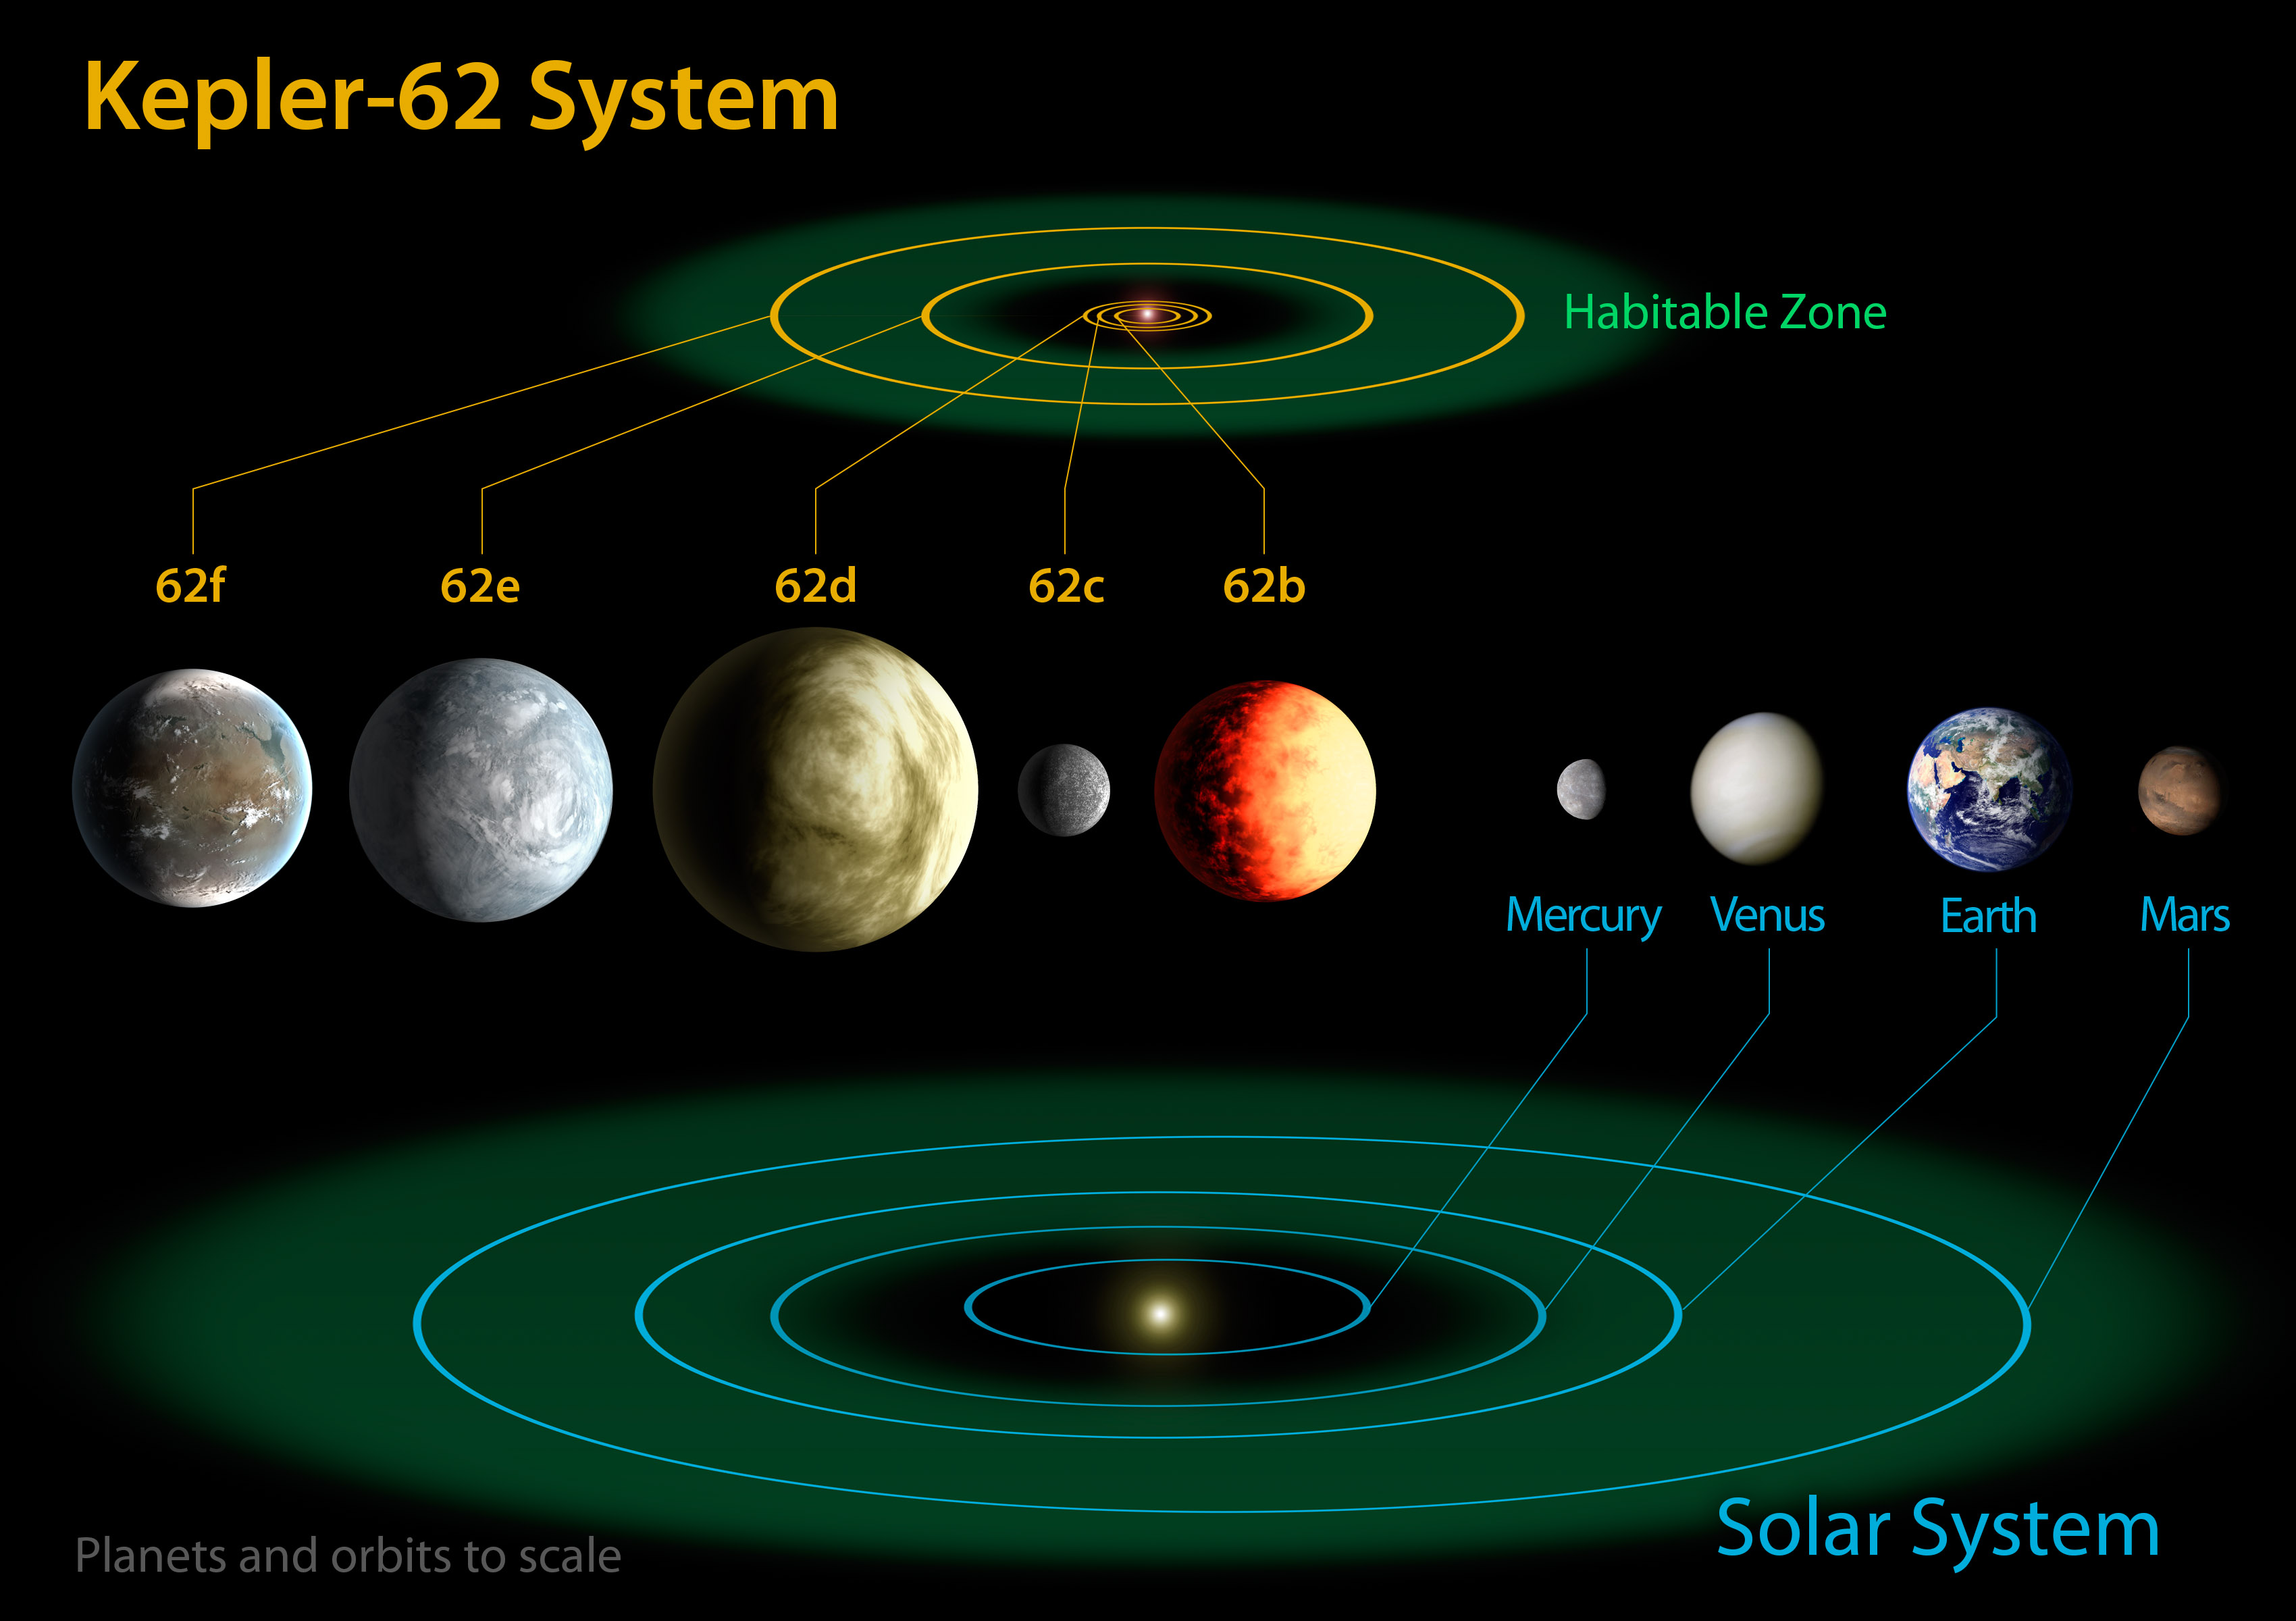
\includegraphics[width=230pt]{Kepler62f.jpg}
\end{figure}
\section{Project description}
\par Our objective was to simulate a sample retrieval mission to a potentially habitable exoplanet, where a sample of soil is taken as well as a video and numerous data assessing the probability of Earth-like life existing on the planet.
\par The main goal was to detect life and conditions for it such as concentration of various gases. Those achievements are necessary for the launch to be considered successful. Other goals were to land the Cansat in a predefined location and to broadcast live data and video to our websites. \cite{Websites}
\par Our task was not easy and we have been aware of that since beginning of the project. We knew that not all of the parts will work but we were prepared for that. Our strategy was to fill as much as we could with sensors and other electronic devices so that in case of one sensors failure we would still get a lot of data to be processed. Unfortunately, before the final flight unexpected problems occurred and we did not have enough time to fix them. The most of hardware was working fine, however, because of few substantial mistakes our Cansat did not work at all. These issues and other information about construction are described in following paragraphs.
\subsection{Cansat}
\subsubsection{Materials and structural design}
\par The main structural body consists of 6 hull parts, which are 3D printed and is screwed to each other. The hull is round at the top and consists of four pillars in the remaining space. Four arms made out of carbon rod are attached to the top part in such way that they can easily move themselves into horizontal position. At the ends of the arms there are printed motor holders for secure and tight fit. In the pillars there are 16 batteries providing the whole Cansat with enough power for the flight and measurements.
\par The space inside was filled with various electronic parts. On the top, there is a three-part main circuit board, which is the “brain” of whole Cansat and on which most of sensors are placed. In the lower inside area there is a flight controller, a power regulator, a servo for soil sample and camera which broadcasts the whole flight to the ground station. All of these parts were  connected to a vertical PCB interconnecting everything and attaching it to the main PCB.
\par According to our plan GSM module should be sited near the flight controller for receiving other data. However, we are convinced that using GSM does not make any sense with our mission, landing on exoplanet.
\begin{figure}[!h]
\centering
\caption{Block diagram}
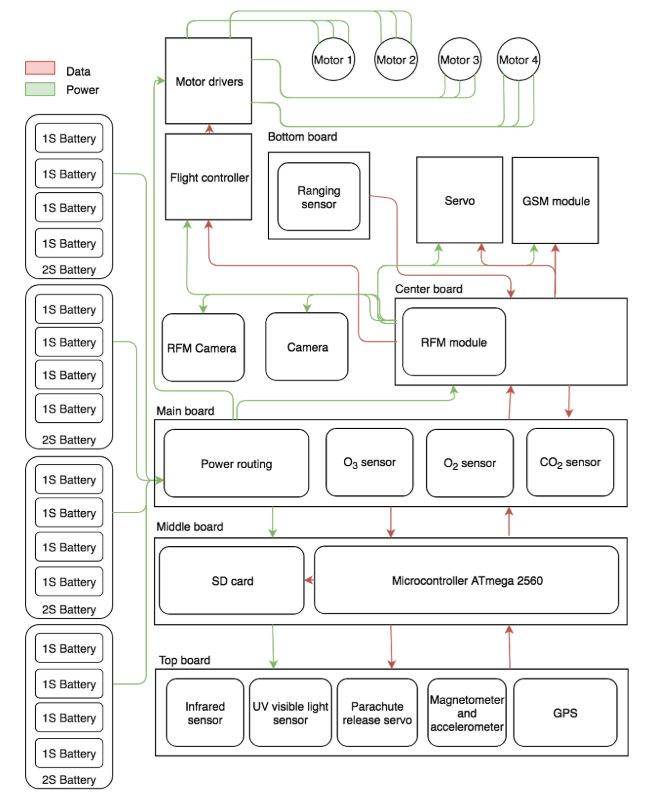
\includegraphics[width=230pt]{block_diagram.JPG}
\end{figure}
\subsubsection{The main hardware issues}
\par During construction and testing of our Cansat there kept repeatedly occurring severe issues with I2C interface devices. The fact that all these problems always disappeared spontaneously made them very difficult to diagnose and we were not able to detect the main reasons of the occasional misbehaviour of our Cansat. All these led to the critical moment, when, despite many successful tests, the SPI and I2C interfaces stopped responding a few moments before the final launch. Due to this, we lost, among the others, also sensors (connected to I2C) measuring the altitude, velocity, acceleration and proximity, which were necessary for the autonomous drone landing system. Secondly, despite values from analogue sensors still being measured, we were unable to store or transmit any data because of not working transmitter and SD card (connected to SPI). 
\par Despite precise tests and measurements after the launch, such as connecting every single sensor separately to the Arduino and checking it or searching for any possible shorts, we could not identify the concrete issue.
\par The most probable explanation is a short between mentioned interfaces which was caused by a metal fragment from cutting PCBs or a thin piece of wire fallen in the circuit. This theory is also supported by the fact that there were found a few metal fragments in drone motors.
\par According to mentioned information, the main reason is in general the insufficient precision during the manipulation with Cansat and avoiding impurities.
\subsubsection{Recovery system}
\par The descent should have been controlled using 4 electric motors which combined have about 640 g of thrust at max. We had planned that arms holding the motors put themselves from resting position into flight position. This system was tested three months before the final competition with receiver placed in Cansat, which was connected to transmitter controlled by a person. The test was successful and Cansat was able to fly with someone’s help. 
\par The stabilisation was possible thanks to flight controller F3 SP Racing, which is normally used as a main board for racing quads. It contains only an accelerometer, gyroscope and tuned software needed for communication with ESCs (Electric speed controller). All of these parts, motors as well, were made for quad racing and for this reason our satellite had enough power and a fast response.
\par After stabilisation motors should have slowed down the descent and then it would have been navigated by GPS, barometer for precise height and magnetometer. Right above ground, about 5 meters, Cansat would have slowed down even more for soft touchdown.
\par Before flight we were forced to use parachute only because of the problems mentioned above. For some reason GPS became very unreliable since we landed on Azores. From our point of view, it could be damaged during flight to Azores or during checking our luggage in. After the issues with  I2C interface the other important sensors like accelerometer and proximity sensor became non-functional. Without all these sensors we were unable to determine the exact location of our Cansat and flight with propellers was impossible.
\begin{figure}[!h]
\centering
\caption{Exploded view}
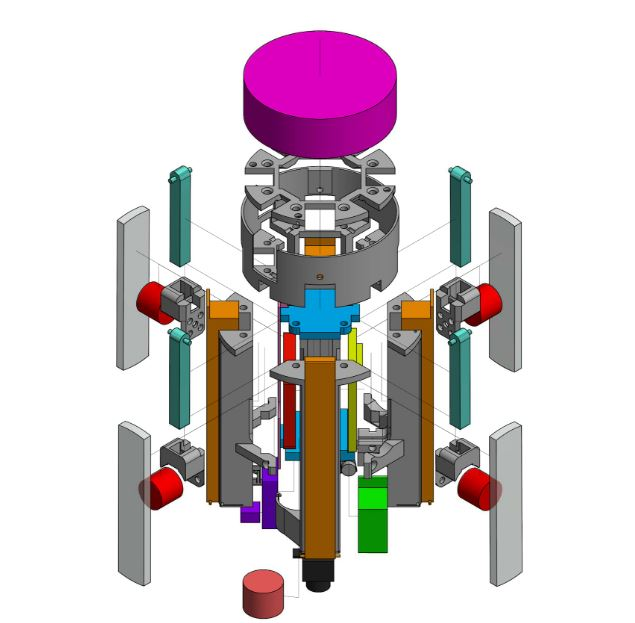
\includegraphics[width=230pt]{exploded_view.JPG}
\end{figure}
\subsubsection{Double emergency landing system}
\par What we would like to highlight is our solution of the emergency landing. To explain our emergency system it is necessary to mention, that the logics based on ATmega and the flight-controller are two separated systems, so that any error on one of them can’t influence the other one. 
\par In case of failure of any “drone part”, such as motors, regulator or already mentioned flight-controller, the logics detect this misbehaviour (e.g. to high descend velocity), it stops the motors and releases the parachute using a small servo placed near the top board. After that the Cansat would be able to land safely. That is how our primary emergency system works.
\par The secondary emergency landing system is activated when the logics stops working. In this case the flight-controller overtakes the control of motors, sets a stable throttle for slow descending and lands, using its own embedded gyroscope.
\subsubsection{Final electrical design}
\par The CanSat contained nine custom PCBs. In the top part three parallel round PCBs were located. The top one contained sensors:
\paragraph{GPS ublox neo-m8n}This  module contains two independent parts: compass, which communicates via I2C and GPS module connected to serial port. It has also its own memory to store the last recognised location, so it can synchronise faster when initiated. It is very important sensor for autonomous landing.
\paragraph{Humidity sensor SI7021}Humidity is important factor when investigating the possibility of life. Using I2C inteface. Its precision is $\pm$ 3$\%$ RH (max), 0–80$\%$ RH
\paragraph{Light sensors TSL25911 (visible and infrared)}From observing received light in different altitudes is possible to estimate content of the atmosphere. Using I2C interface.
\paragraph{VEML6070 (ultraviolet)}UV light is dangerous for many forms of life and its measuring in different altitudes give us a chance to estimate content of the atmosphere. Using I2C interface.
\paragraph{Pressure and temperature sensor MPL3115}Combined with other data (e.g. G), pressure can be used to count the thickness of the atmosphere and the right temperature is necessary for planet’s habitability. Using I2C interface. Precision ADC resulting in 0.1 meter of effective resolution.
\paragraph{Magnetometer and accelerometer LSM303AGRTR}This sensor is essential for the autonomous landing system. Using I2C interface.
\par On the middle board there were an ATmega2560 microcontroller and a SD card. The lower board took care of power routing and regulation and also contained gas sensors:
\paragraph{MG812 (CO\textsubscript{2})}Range: 350-10000ppm CO\textsubscript{2}
\paragraph{MEO2 (O\textsubscript{2})}Range: 0-25\%vol
\paragraph{SP3-61 (O\textsubscript{3})}Range: 100ppb O\textsubscript{3}
\par Levels of these three gasses are very important when investigating the habitability of the planet, especially for atmosphere’s breathability and the greenhouse effect. Then our Cansat was equipped  with one external sensor:
\paragraph{Distance laser sensor VL53L0X}This sensor helps with soft touchdown of Cansat, because GPS and barometer are not accurate enough. Using I2C interface.
\par Batteries were connected four in parallel on each pillar PCB which have connectors for charging and connection. To the bottom of the main PCBs was connected a vertical PCB to which all modules or devices were connected. In that space motor drivers, flight controller, gamma detection board, sample collection servo, and camera were located.
\par Sixteen 1S LiPo batteries are used in a 2S (7.4V) configuration. Each battery gives 200 mAh at 3.7V and allows 35C discharge. That amounts to 1600mAh at 7.4V and 280C discharge. All logic electronics had been expected to draw up to 1A and the motors draw 15A on average. Because we decided to use only parachute we had much more energy than we had supposed. After the flight the voltage of one battery cell was at 4,1 V (maximum charge is 4,2 V). 
\par The PCBs were designed using KiCAD. All schematics are available at our GitHub/../Circuit \cite{Git-Circuit} and a detailed list of parts is located at our website. \cite{Websites}
\subsubsection{Sofware design}
\par The program initializes and then keeps running in loop where it measures data from sensors and GPS, based on GPS controls motors speed and CanSat’s direction and transmits data to ground station.
\par If any component fails, a watchdog is triggered to reset the microcontroller and the faulty component is disabled during initialization. If this happens during flight or any component required for flight is disabled the program jumps to parachute flight as a security precaution, disabling the motors and releasing the parachute. This happens within five seconds of a fault causing the program to freeze.
\par All Cansat software is written in Arduino code based on C++. We used a huge amount of libraries for which we thank their creators. We used CLion IDE, Atom editor, Arduino IDE and PDE (Processing Development Environment). Every bit of our code or code we used has GNU GPL license and it is available at our GitHub. \cite{Git - Code}
\begin{figure}[!h]
\centering
\caption{Software decision tree}
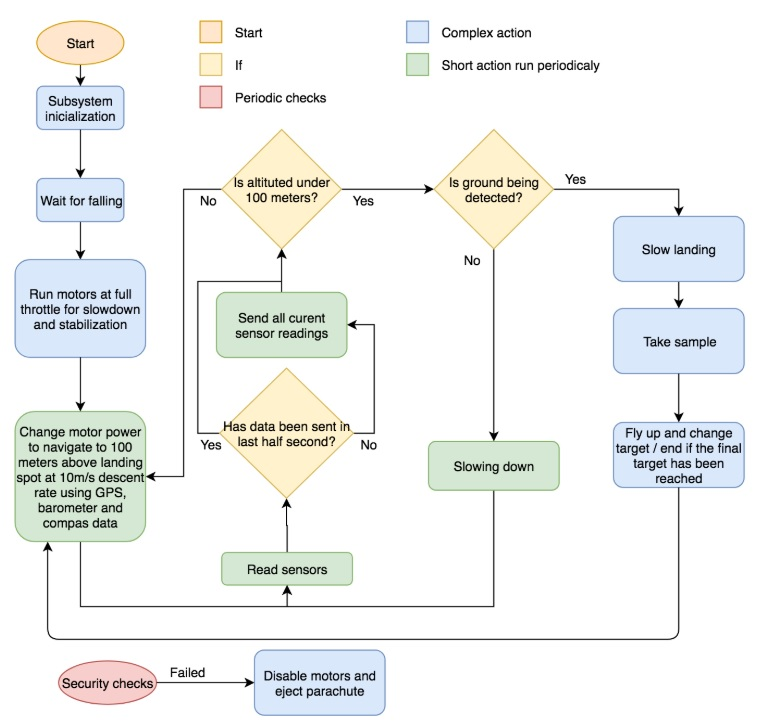
\includegraphics[width=230pt]{decision_tree.jpg}
\end{figure}
\subsection{Ground station}
\subsubsection{Ground support equipment}
\par The ground station is split up between two laptops. One is receiving through an analogue antenna the video feed from onboard camera. The emitting power of video transmitter was approximately 200 mW and for two kilometers we needed more. However, we were limited by space in our satellite and by maximum power of batteries. For this reason, we decided to use diversity receiver with three patch antennas (14 DBI). That set should work to distance over 2,5 km. The receiving video was saved locally on the computer. We had also planned to stream the video to our Youtube channel for fans but there was no stable internet connection on the spot of the flight. 
\par The second laptop was connected to Arduino Nano via USB connection and runs a processing sketch which listened to Arduino’s serial. The sketch processes the input data, saves all communication and logs errors were capable of sending data to our web page where it is stored as a backup and graphed for live inspection. The Arduino is running a simple script for receiving data from Yagi antenna which we made ourselves and printing it to the serial.
\section{Data measurements and processing}
\subsection{Theory}
\subsubsection{Basic variables}
\paragraph{Gravitational acceleration}If we average each partial acceleration measured and calculate a Pythagorean sum of those, we should get gravitational acceleration. The problem is that the axis can not rotate during measurements. The data from a gyroscope is not reliable enough due to low sampling level. Therefore only data measured on the ground can be used.
\paragraph{Atmospheric density} The vertical gradient of pressure is linear to the density of the air:\\
\begin{equation}
    \rho = g \frac{dp}{dh}
\end{equation}
\paragraph{Atmospheric composition} \label{basic}
From Tinetti's analysis \cite{Tinetti} we obtained the general composition of the exoplanet atmosphere, depending on the variables we know or can compute:
\begin{figure}[!h]
\centering
\caption{Exoplanet composition}
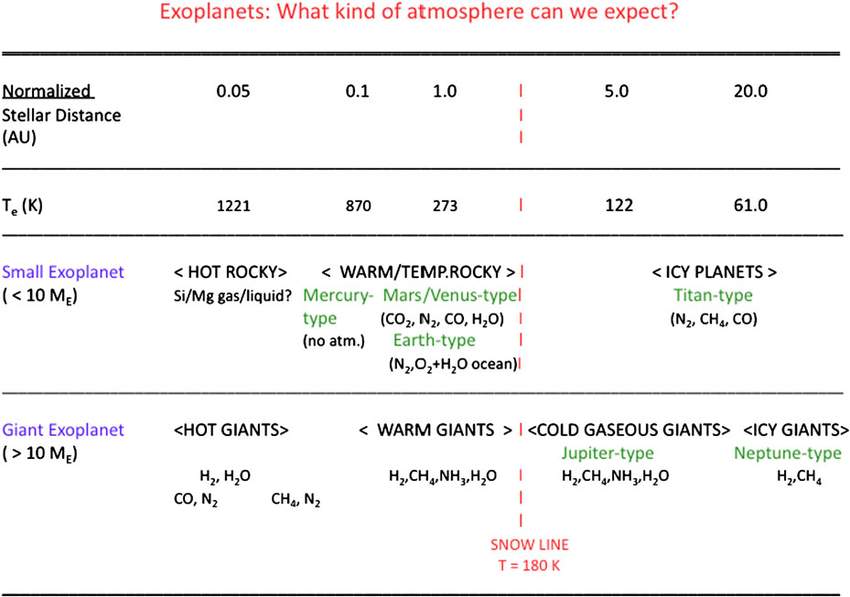
\includegraphics[width=230pt]{A-simple-classification-for-the-atmospheric-composition-of-exoplanets-based-on-their.jpg}
\end{figure}
\paragraph{Mass of the planet} The mass of the planet can be obtained using Newton's law of gravity:\\
\begin{equation}
    M = \frac{g R^2}{G}
\end{equation}
\paragraph{Atmospheric density} The vertical gradient of pressure is linear to the density of the air:\\
\begin{equation}
    \rho = g \frac{dp}{dh}
\end{equation}
\paragraph{Average molecule mass} We can derive the number of particles per unit of volume from the ideal gas law and from that and density the molecule mass:\\
\begin{equation}
m_{molecule} = \frac{\rho}{N} = \frac{\rho k_B \tau}{p}
\end{equation}
\paragraph{Mass of the atmosphere}
From Trenberth's analysis \cite{Trenberth} we get an equation to calculate the mass of atmosphere:
\begin{equation}
m_{atm} = \frac{2\pi R^2 f}{g} \int_{-\frac{\pi}{2}}^{\frac{\pi}{2}} [p_s(\theta)]cos\theta d\theta
\end{equation}
where $f$ is the net effect of the shape of the planet and gravity variations with height and latitude but its value is very close to one and therefore at our level of precision negligible, as we cannot determine it exactly, $R$ is radius of the planet, $g$ is gravitational acceleration and $[p_s]$ is the average surface pressure. \subsubsection{Size of the atmosphere}
The two major factors limiting the size of the atmosphere, that is the altitude, at which an average molecule will escape into space, are the following:
\paragraph{Speed of molecules exceeding escape velocity} Even the top of the atmosphere rotates with the planet so the speed of some molecules is at least the sum of the rotational velocity and mean quadratic velocity of the molecules. As the velocity of molecules depends on temperature, which we did not measure a guess must be made. As there is very low density at the top of the atmosphere, the thermal conductivity can neglected. The top of the atmosphere is mostly heated by highly energetic particles from deep space (they do not originate in the star so their concentration can be considered constant in nearby stellar systems. Therefore we can say the temperature there is the same as at the top of the atmosphere of the Earth with the expected precision of a 100 kelvins (it propagates only as a small deviation).
\paragraph{Magnetosphere} We can expect form figure \ref{mag} and from Maxwell's second equation that the size of magnetosphere will be roughly linear with size and from the figure that a magnetic field at least third of the size of Earth's one will be good enough.
\begin{figure}[!h]
\centering
\caption{Earth magnetosphere under solar wind pressure}
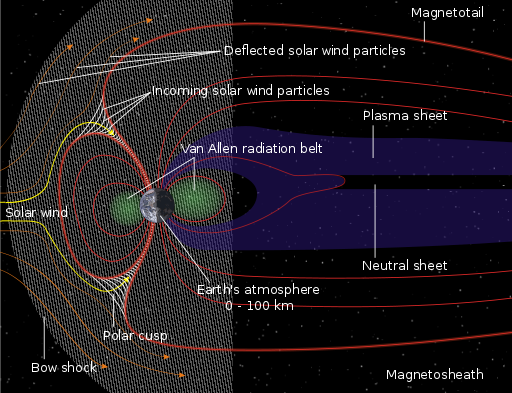
\includegraphics[width=250pt]{mag.png}
\label{mag}
\end{figure}
\begin{align}
v_{escape} &= v_{rotational} + v_{mean quadratic}\\
\sqrt{\frac{2MG}{r}} &= \frac{2 \pi r}{T_{rotation of planet}} + \sqrt{\frac{3 k_B \tau}{m_{molecule}}}
\end{align}
\paragraph{Solar constant}
\begin{align}
P = \frac{k_B*4*\phi*r_{star}^2*T_{star}^4}{d^2*4*\phi}
\end{align}
where $k_B$ is Boltzmann's constant, $r_star$ is Parent star's radius, $T_star$ represents parent star's surface temperature in kelvins, d represents distance between the star and the place, where we measure solar constant. Basically, it is the radiance of an absolutely black body on an area of 1 $m^2$ per sphere of a given radius.
\paragraph{Temperature without greenhouse effect}
\begin{align}
T = \bigg(\frac{P}{4*k_B} * (1-A)\bigg)^{0.25}
\end{align}
where A is albedo, which is the variable that tells us what amount of light on a scale from 0 to 1 reflects the body. The rest variables and constants were mentioned above. 
The resulting temperature will be in kelvin of course.
\subsubsection{Greenhouse effect}
\par This is a very complex issue, first it is necessary to calculate spherical variables depending on the position on Earth and time. We then move on to more complex purely physical calculations.
\par First, we calculate when the sun passes through the local meridian.
\begin{align}
t_{noon} = 12 + t_{delta} + \frac{\lambda+Z*15}{15}\\
\end{align}
\par where $t_{delta}$ represents the changes made by the law as summer or winter time, at Azores it was +1, then $\lambda$ is longitude value. And Z represents time zone, Azores belong to UTC time zone. The whole idea is that the Earth rotates about 24 hours around its axis (360 degrees). Thus, the angular distance from the meridian that defines the time zone can also be considered as a time distance. 
\par Changes in the angle of the bodies in the sky in the horizontal direction are linear, as it is based on the rotational speed of the Earth, which is constant. We will use this fact in further calculations. These inconsistencies can usually be neglected, but the time zone of Azores does not correspond to its geographical location, and therefore it is necessary to consider this matter and calculate when the astronomical noon is taking place. It is then necessary to compute the maximal declination which is the key for us, in addition it provides an important fact how long does it last between the sunrise and sunset.
\begin{align}
\delta = 23.45*\sin(0,98*DD+29,7*MM-109)
\end{align}
DD represents the day of the month and the MM month of the year. Since the earth axis performs precision and nodding movement, our calculations are based on an approximation according to our national standard ČSN 730581.
\begin{align}
\delta_{max} = 90-\phi+\delta
\end{align}
where $phi$ is latitude. This relationship gives us a maximum declination on a given day at a given place on the ground. This is derived from the basic trigonometry. Then we can calculate length of the day, our calculations are based on the Giesen's \cite{Giesen}.
\begin{align}
t_{rise} = 12 - \frac{arccos(-\tan(\phi)*\tan(\delta))}{15} \\
t_{set} = 12 + \frac{arccos(-\tan(\phi)*\tan(\delta))}{15}\\
t_{daylight} = \frac{2*arccos(-\tan(\phi)*\tan(\delta))}{15}
\end{align}
where $t_{rise}$ is a time of sunrise, $t_{set}$ time of sunset and $t_{daylight}$ represents length of the day. 
Now we can calculate how much energy a $m^2$ has taken over the time from sunrise to measurement time.
\begin{align}
\delta_{time} =\frac{\delta_{max}}{t_{noon}-t_{rise}}*(t-t_{noon})
\end{align}
or (for measurement after real noon)
\begin{align}
\delta_{time} =\frac{\delta_{max}}{t_{set}-t_{noon}}*(t_{set}-t)
\end{align}
where t is current time of measurement. As it was mentioned above, the angular velocity is linear, so the height of the Sun is determined for some time as the ratio of the time elapsed versus the total time. Surface receives energy based on sine function:
\begin{align}
E =(1-A)*P*3600*(t-t_{rise}) \int_{0}^{\delta_{time}} \sin(x)
\end{align}
or (for measurement after real noon)
\begin{align}
E =(1-A)*P*3600*(t_{set}-t) \int_{0}^{\delta_{time}} \sin(x)
\end{align}
where A is albedo and P is so called solar constant, both is used and explained above in 3.9 and 3.10. Integral solution is: 
\begin{align}
\int_{0}^{\delta_{time}} \sin(x) = \cos(0) - \cos(\delta_{time})
\end{align}
if we have received energy on $m_2$, so we can calculate how this energy changed ground temperature.
\begin{align}
t_{ground} =t_{air} - \int_{a}^{b} \cfrac{1}{\frac{E*(1-A_{clouds})}{\rho*c}}
\end{align}
where $\rho$ is density of the ground, c is specific heat capacity, both of these values for final calculation are drawn from TBZ catalogue \cite{TBZ}. $t_{air}$ represents temperature measured at the ground level, $t_{ground}$ is our calculation of the temperature of the ground without heating by the parent star. $A_{clouds}$ is a number of albedo style (from 0 to 1), which represents how much energy from the sun the cloud reflects on his way to the surface. We have to think that the day when it is measured can be overcome. Cloud rate estimation can be determined from both our spectrographic analysis and the camera that the satellite carries. Consideration of this factor significantly improves the analysis. Taking into account the state of the sky on the day of the final flight and the work of Sigmund Fritz \cite{Fritz}, we consider albedo of the clouds in the final calculation as 0.55. Integral solution is:
\begin{align}
t_{ground} =t_{air} - \frac{1}{\frac{E*(1-A_{clouds})}{\rho*c}}*\frac{\ln{b}-\ln{a}}{b-a}
\end{align}
by using the integral and dividing the boundaries we get an average value. Here, it is necessary to realise what the integral means. From the hyperbolic function (it is logical that with the depth the average value will be closer to the air temperature, if we neglect the lower heating of the soil, it is the passage of the energy from the top layer below, respectively in the winter this phenomenon works on the contrary) we obtained the difference of logarithms, zero argument can not be inserted into the logarithm. Why is that so? The boundaries determine the area of the soil, which according to us is warming up and the average tells us then how this area is heated as a whole. Therefore, the soil layer logically can not have zero value, here mathematics and physics are beautifully interconnected. We have therefore chosen a range of 12 to 90 centimetres.
(Our model is available online so you can play with the limits according to your preference.)
\begin{align}
a = 0.12
\end{align}
\begin{align}
b = 0.9
\end{align}
these limits are bounded by stable soil profiles B and C, whose temperature changes with respect to weather, but the change takes more time. This is a good representation of what we are looking for.
\begin{figure}[!h]
\centering
\caption{Soil types taken from work of Tapas Bhattacharyya \cite{Bhattacharyya}}
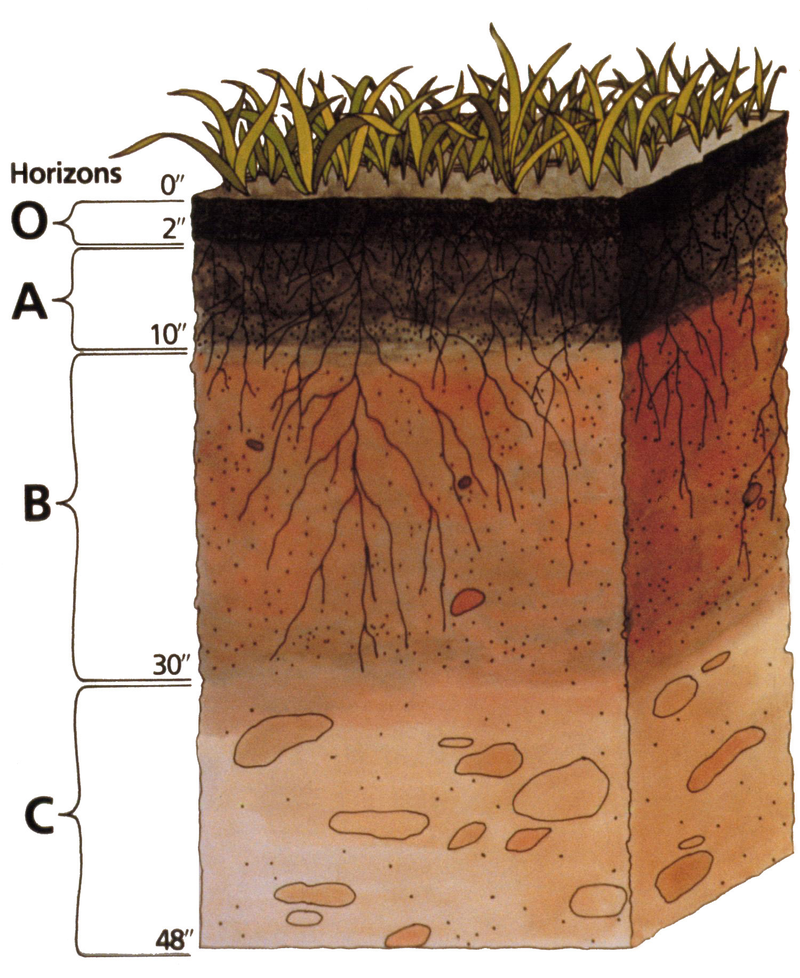
\includegraphics[width=230pt]{Soil.png}
\end{figure}
\par Now we have the soil temperature, useful fact itself, but mainly essential for the final calculation of the greenhouse effect. We use this fundamental equation, which represents energy changes in the atmosphere, based on the greenhouse effect scripts from Harvard \cite{Jacob}:
\begin{align}
\phi*r_{planet}^2*P*(1-A) = \\ 4*\phi*r_{planet}^2*(1-f)*\sigma*T_{ground}^4 + 4*\phi*r_{planet}^2*f*\sigma*T_{air}^4
\end{align}
where A is albedo, P is solar constant. Both was used above. $\sigma$ represents Stefan-Bolzmann constant, $r_{planet}$ is a radius of the planet. From this equation we were able to compute f, which expresses the amount of reflected (longwave) radiation by the clouds back on the ground:
\begin{align}
 f = 2*(1-\frac{P*(1-A)}{4*\sigma*T_ground^4}
\end{align}
like the scripts we used formula for a separate energy balance equation applies to the atmospheric layer:
\begin{align}
f*\sigma*T_{ground}^4 = 2*f*\sigma*T_{air}^4
\end{align}
however they used system of equations differently. The value f is measurable on the global scale and nobody discovers it and uses this calculation to calculate the soil temperature. However, the temperature of the soil has been determined from the calculation by another method and thus we can very precisely determine the value of f, which is not very common. In other words, local measurement allowed us to have a variable valid for the entire planet.\par
\begin{figure}[!h]
\centering
\caption{Energy changes according to the scripts of Harvard}\cite{Jacob}
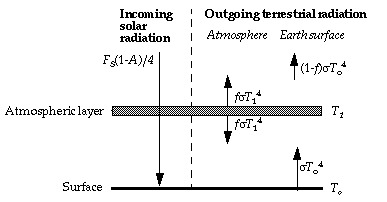
\includegraphics[width=230pt]{bookchap7-25.jpg}
\end{figure}
As a final result of these all calculations we know f, however to get this result we need to derive a lot of variables that also provide us with interesting data - such as a square meter energy flow, which is important information for using solar panels as well as an estimate of the nature of life on the planet.
\paragraph{CO\textsubscript{2} equivalents}
\par The effect of a given gas on the greenhouse effect can easily be expressed in terms of carbon dioxide. Given this significance and the concentration of gas as a weighted average, it is possible to determine the extent to which the gas participates in the whole process. The only unknown is water vapour whose volume in the air is constantly fluctuating, but global warming is a global phenomenon \cite{Geocraft}, so we compared the state without steam, and then its coefficient was 0.72 in order to distort the results as little as possible other gases. However, the results without water vapour calculations are certainly reported and conclusive. According to Strobel, the coefficients are as follows \cite{Strobel}:
 \begin{tabbing}
    Gas ~~~~\= CO\textsubscript{2} equivalent ~~~~
    \= 34 \kill
    \bfseries  Gas\>\>
    \bfseries CO\textsubscript{2} equivalent\>\\
    $CO_2$ \>\>1.0\\
    $H_2O$ (vapour) \>\>0.72\\
    $CH_4$ \>\>80\\
    $O_3$ \>\>1000\\
    $NO_2$ \>\>300\\
    \end{tabbing}
\par It should be noted that the tropospheric ozone equivalent is 1000 units of $CO_2$, but due to the short lifetime, the value on the 20-year scale is only 62 to 69 units. \cite{Ozone co2e} We decided to use 1000 units for our calculations, so results represents properties of the atmosphere are exactly at the moment of measurement.
\subsubsection{Spectroscopic measurements}
We are using spectroscopic sensors with sensitivity functions depicted in Appendix 2. The theory often deals only with wavelengths 280-890 depicted there.
\paragraph{Thermal radiation at the top of the atmosphere} The spectral radiance is specified using Planck's law. As spectral radiance is radiant flux per wavelength per steradian, we can multiply it with the solid angular size of the star to calculate the spectral radiant flux at the ground if there were no atmosphere.
\begin{align}
\Phi_{e}(\lambda) &= B_{\lambda}(\lambda) \Omega_{Star}\\
\Phi_{e}(\lambda) &= \frac{2 hc^2}{\lambda^5}\frac{1}{ e^{\frac{hc}{\lambda kT}}-1} 4 \frac{\pi R_{star}^2}{4 \pi r_{planetary orbit}^2}\\
\end{align}
\paragraph{Luminous flux} Luminous flux is what the sensors measure. To do the analysis, first we have to calculate what they should measure if there were no atmosphere:
\begin{equation}
\Phi_v = 683.002 \frac{lm}{W} \int^{\infty}_0 \overline{y}(\lambda) \Phi_{e,\lambda}(\lambda)\, d \lambda
\end{equation}
where $\overline{y}$ is luminosity function.
\paragraph{Absorption} For every gas there is a function of wavelength that gives absorption cross section. Then we can calculate the absorbed portion of light at that wavelength.
\begin{align}
\frac{dN}{N} &= -dx n \sigma\\
N(\lambda) &= N_0(\lambda) e^{ -x \sigma(\lambda)}
\end{align}
Where $n$ is number of absorbing particles per unit volume and $N(\lambda)$ is the number of photons with wavelength $\lambda$. We can do the same for radiant flux:
\begin{align}
\Phi_{e} &= \Phi_{e0}(\lambda) e^{ -x \sigma(\lambda)}
\end{align}
If we set $n$ as particles per unit volume (cubic meter in SI) at sea-level (we use values from Earth because this is just for comparison), than $x$ would be the height of the layer of gas if it were pure and at sea-level. That is useful for comparison as for example ozone layer thickness is often given as such variable. It will be useful to determine the total masses of the gases. To do that we will suppose that composition of atmosphere is constant with height. We will also use the isothermic model for the atmosphere, because although it adds extra air in comparison with other models, there is air practically orbiting the planet (for Earth that is the case for the exosphere) which is ignored in the models based on the derivative of pressure. We need that to determine the mean spherical surface of the atmosphere. We can use barometric formula as density of air is linear to pressure for isothermic atmosphere.
\begin{align}
m_{gas} &= x_{gas} \rho_{gas} \frac{\int_R^\infty 4 \pi r^2 P_0 e^\frac{-g M (r - R)}{R^* T_b}}{\int_R^\infty P_0 e^\frac{-g M (r - R)}{R^* T_b}}\\
m_{gas} &= x_{gas} \rho_{gas} 4 \pi \Bigg(R \bigg(R + 2\frac{R^*T_b}{gM}\bigg) + 2\bigg(\frac{R^*T_b}{gM}\bigg)^2\Bigg) %vychází 8.9 km vysoko
\end{align}
where $\rho_{gas}$ is density of the gas at sea-level on Earth, it has to be on Earth because the thickness of the layer ($x$) is also a value converted to on-Earth.
\subsubsection{Overall concentration of gases in the atmosphere}
We can choose a few expected gases and determine their concentrations by fitting the calculated data (expected measurements with given concentrations) to the measured. We must also take into account the greenhouse effect and the mass of the atmosphere (the calculated amounts of gas from spectroscopy must add up to the mass of atmosphere).
\subsubsection{Sensor correction}
The sensors measure with decreased sensitivity when light is at an angle, also less light falls on the clouds, we have to calculate for this by dividing the measurement by sine of the angular height of sun above horizon. Near sunset and sunrise this has to be correlated by (arcminutes that have to bee added to the angle above horizon) \cite{refra}:
\begin{equation}
    R = 1.02 \cot \bigg( h + \frac{10.3}{h + 5.11} \bigg) \frac{p}{101} \frac{283}{273 + T}
\end{equation}
\subsection{Transmissivity of clouds}

\

We will try to estimate what proportion of light goes through cloud and what proportion is reflected. Every cloud is composed of big number of water droplets with average radius between $10 \mu m$ and $20 \mu m$. This radius is big in comparison with wavelengths of UV, visible light and IR so we cannot use Reyleigh approximation but we can use geometrical approach. 

\

Water droplet has a radius $R$ and the light has irradiance $E_{e}$.  We shall count refraction and reflection of light on the spherical droplet. Light enters the droplet in distance $r$ from the droplet axis as we can see it in the figure~1.

\begin{figure}[h]
\centering
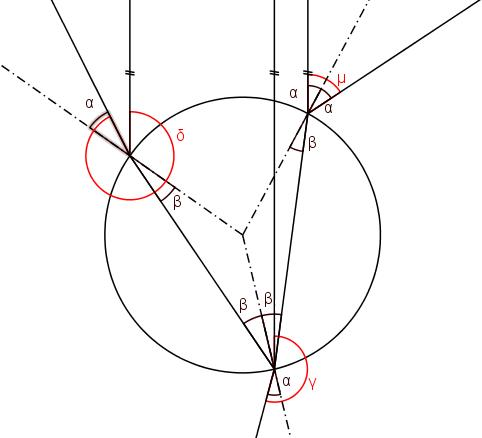
\includegraphics[width=230pt]{droplet.jpg}
\caption{Light in a droplet}
\end{figure}

The angle of reflection is the same as the angle of incidence according to \textit{the law of reflection}, for angle of refraction holds the \textit{Snell's law}. One part of light is reflected and the rest is refracted. The ratio between these parts is described by \textit{Fresnel equations}. Light striking the droplet is randomly polarized so we can resolve it into two equally big components with $s$ and $p$ polarizations. The Fresnel equations are:
$$A_{s}={\left(\frac{\sin{(\alpha-\beta)}}{\sin{(\alpha+\beta)}}\right)}^2$$
$$A_{p}={\left(\frac{\tan{(\alpha-\beta)}}{\tan{(\alpha+\beta)}}\right)}^2$$
$R_{s}$ and $R_{p}$ denote fraction of power of reflected light in respective polarizations, $\alpha$ angle of incidence (which is the same as angle of reflection) and $\beta$ angle of refraction. Fractions of refracted light obviously are
$$B_{s}=1-{\left(\frac{\sin{(\alpha-\beta)}}{\sin{(\alpha+\beta)}}\right)}^2$$
$$B_{p}=1-{\left(\frac{\tan{(\alpha-\beta)}}{\tan{(\alpha+\beta)}}\right)}^2$$
In figure 1 we can see path of light with marked angles of incidence, reflection and refraction. The light is reflected and refracted infinite number of times, but from practical reasons we can take into account only three refractions and reflections (in simulation it turns out that almost 99\% of light exit the droplet during these three refractions and reflections).
We made a simulation using Microsoft Excel. For each distance $r$ from droplet axis (with certain step), we counted the dependence of radiant flux on angle under which the light exit the droplet and after counting for $r\in\left( -R, R\right) $ where $R$ is radius of droplet we obtained the function of radiant flux
$$\Phi_{e}(r, \mu, \gamma, \delta)$$
where $\mu$, $\gamma$ and $\delta$ are the angles under which the light exit the droplet after first, second and third reflection (refraction).

\begin{figure}[!h]
\centering
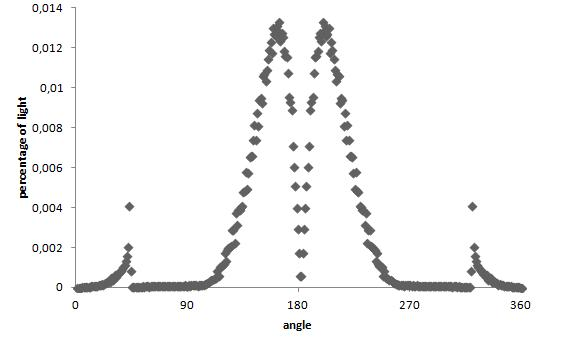
\includegraphics[width=250pt]{dr.jpg}
\caption{Light in a droplet}
\end{figure}

We simplified this model and counted only the percentage of light which exit the droplet under angle between $(0^{\circ},90^{\circ})\cup(270^{\circ},360^{\circ})$ so it exit upwards and percentage of light which passes through droplet downwards under angle between $(90^{\circ},270^{\circ})$.
Our numerical simulation says, that the percentage of transmitted light is
$$\tau\cong94.8\%$$
This number does not depend on wavelength of light and not even on radius of the droplet.

\

How many droplets will the light ray hit after entering the cloud from above? As we can see in figure 2 the direction of the light ray after going through the droplet does not differ very much from original direction (maximum of light is refracted under 20$^{\circ}$). Thus, we can assume that the ray hits only droplets which are above each other. Each droplet transmits 94.8\% of light and 5.2\% is reflected. There are $n$ layers of droplets in one cloud. This system is in principle the same as the system of one-way mirrors. 

Let us consider two one-way mirrors. Incident ray has the intensity $I$. The transmissivity of both mirrors is $\tau$. Thus the part of light which passes through two one-way mirrors system is $\tau^2 I$. On the second mirror, $\tau(1-\tau) I$ is reflected. Then from the first mirror $\tau(1-\tau)^2 I$ is reflected and through the second mirror passes $\tau^2(1-\tau)^2 I$. We can see a sequence: $\tau^2 I$, $\tau^2(1-\tau)^2 I$, $\tau^2(1-\tau)^4 I$ ... The sum of this infinite sequence divided by $I$ is the transmissivity.
$$\Theta=\tau^2+\tau^2(1-\tau)^2+\tau^2(1-\tau)^4+\cdots=\frac{\tau^2}{1-(1-\tau)^2}=\frac{\tau}{2-\tau}$$
Now let us count the system of n one-way mirrors. Let the transmissivity of $n-1$ mirror be $\Theta$, then for the part of light which passes through $n$ mirrors holds (only slightly different from previous case):
$$T=\Theta\tau+\Theta\tau(1-\Theta)(1-\tau)+\Theta\tau(1-\Theta)^2(1-\tau)^2+\cdots=\frac{\Theta\tau}{1-(1-\Theta)(1-\tau)}=\frac{1}{\frac{1}{\Theta}+\frac{1}{\tau}-1}=\frac{1}{\frac{1}{\Theta}+\frac{1-\tau}{\tau}}$$
Using induction:
$$T_1=\frac{1}{\frac{1}{\tau}+\frac{1-\tau}{\tau}}$$
$$T_2=\frac{1}{\frac{1}{\tau}+\frac{1-\tau}{\tau}+\frac{1-\tau}{\tau}}$$
$$T_3=\frac{1}{\frac{1}{\tau}+\frac{1-\tau}{\tau}+\frac{1-\tau}{\tau}+\frac{1-\tau}{\tau}}$$
$$T_n=\frac{1}{\frac{1}{\tau}+n\frac{1-\tau}{\tau}}$$

System of $n$ one-way mirrors has the transmissivity
$$T=\frac{\tau}{n-\left( n-1\right) \tau}$$

\

Let us count number of layers $n$ for real situation and then make a comparison of our case with real number of layers.
There are $n$ layers in the cloud of height $H$. Because the cross section of droplet is $\pi R^{2}$ the volume is $V=\pi R^{2}H$ and the mass of droplets in this volume is $m=n m_{0}=\frac{4}{3} \pi \rho_{0} n R^{3}$. The density of water in cloud is hence
$$\rho=\frac{m}{V}=\frac{4}{3} \frac{nR}{H} \rho_0$$
This parameter is experimentally measured and for average cloud (cumulus mediocris cloud) is has the value 1 $g/m^3$. Average cloud height is around 1000 $m$, average radius of droplet $15 \mu m$ and the density of water is $\rho_{0}=1000 kg/m^3$. Thus the indicative number of layers is $n = 12$. For this $n$ is the transmissivity 42\%.
For our case the transmissivity of clouds is 70\%, thus number of layers is $n = 8$.
\

We discovered that the cloud absorbs certain proportion of light irrespective of wavelength (in area of our interest 200-900 nm). In our case cloud can make very good correction of irradiance in our spectroscopic measurement.
\subsection{Determining errors}
\subsubsection{Measured variables}
\paragraph{Constants} Some of the measured variables are practically constant at the reached altitudes. They are gravitational acceleration, the spectroscopic variables and gas concentrations (except relative humidity). Here we calculate the arithmetic mean and the standard deviation of arithmetic mean. As some sensors output a near constant value (for example when they have a really long reaction time) the standard deviation would be quite small if not zero. Than we have to add an instrument error (we will add it to the standard deviation using Pythagorean addition). It is most significant in the gas sensors but as their datasheets don't provide the information and because it increases over time, we have to make an educated guess there. We multiply it by Student's coefficient for 99.9\% and the number of measurements of the specific variable. Therefore if any value that is measured on Earth or calculated from those data, the reference value should be within the deviation of the measured/calculated value. If it isn't we know with 99.9\% probability that there is a systematic error that caused it to deviate.
\paragraph{Variables linear with height} There is also a number of variables that change linearly with height. They are pressure, temperature and relative humidity. We calculate the slope and zero-intercept and the deviation. The deviation is equivalent to standard deviation for the constants, so we can do same operations with it.
\subsubsection{Calculated variables}
During calculations 
\subsection{Data measured}
As our CanSat stopped functioning just before launch, we are using data of the Irish team and our data measured on the ground where the Irish CanSat didn't contain the necessary sensors. The data measured on the ground is taken to be constant with altitude, which is likely for all the variables at the reached altitudes.
\subsection{Data obtainable from Earth}
\par These data about Kepler-62-f was measured by the Kepler probe based on the eclipse detection method. We also use this data in our models: \\\\
Radius - 1.41 radius of Earth\\
Mass - from 2.5 to 3 Earths\\
Semi-major axis - 0.718 AU\\
Circulation time - 267,291 earth days\\
Tilt slope - 89.90 degrees
\par
As we have these data for the target planet, we will use their equivalents for Earth while simulating the mission on Earth.
\subsection{Results}
\subsubsection{Variables linear with height}
\begin{figure}[!h]
\centering
\caption{Full range of measured temperature}
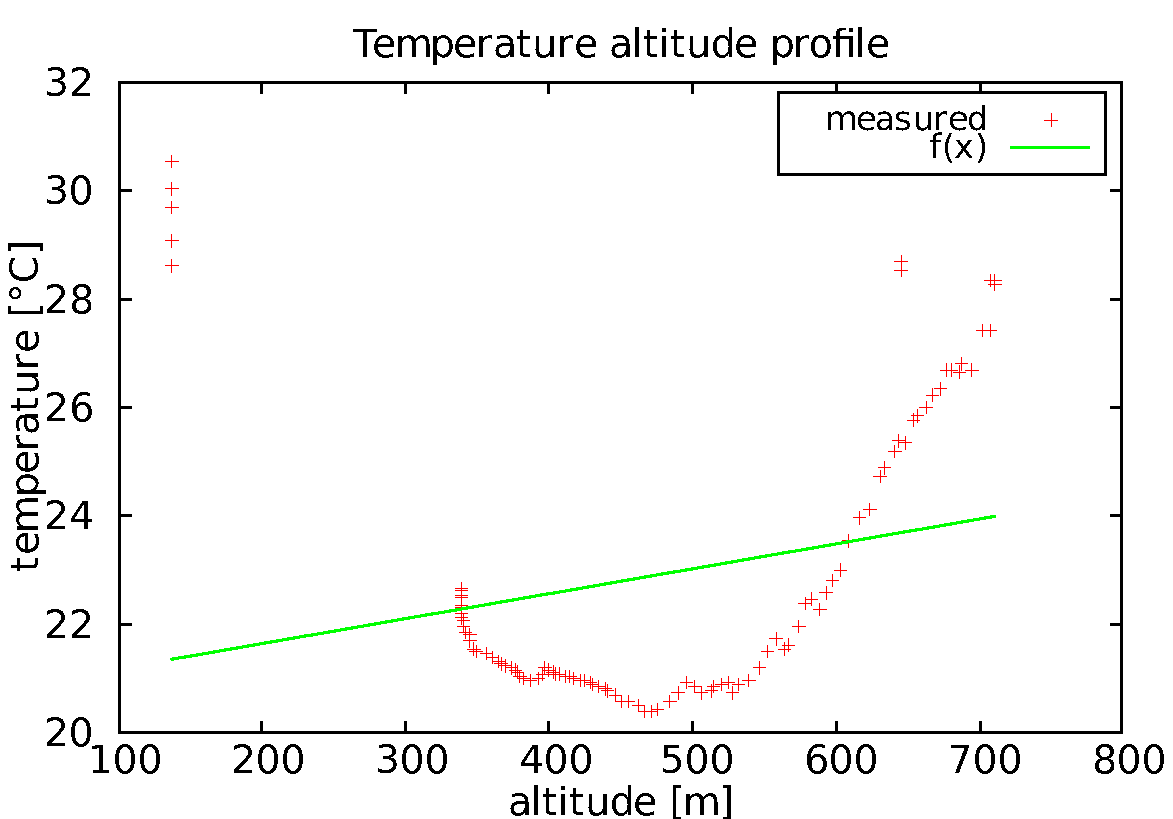
\includegraphics[width=250pt]{temp_before.pdf}
\label{temp1}
\end{figure}
\paragraph{Temperature.} In figure \ref{temp1}, there is a problem that if stationary, sunlight causes the CanSat to heat up. When it moves this effect is still present but hopefully negligable. To have more accurate result, we have to remove those data-points that deviate too much. From that we get figure \ref{temp2}.
\begin{figure}[!h]
\centering
\caption{Non-deviating data-points of measured temperature}
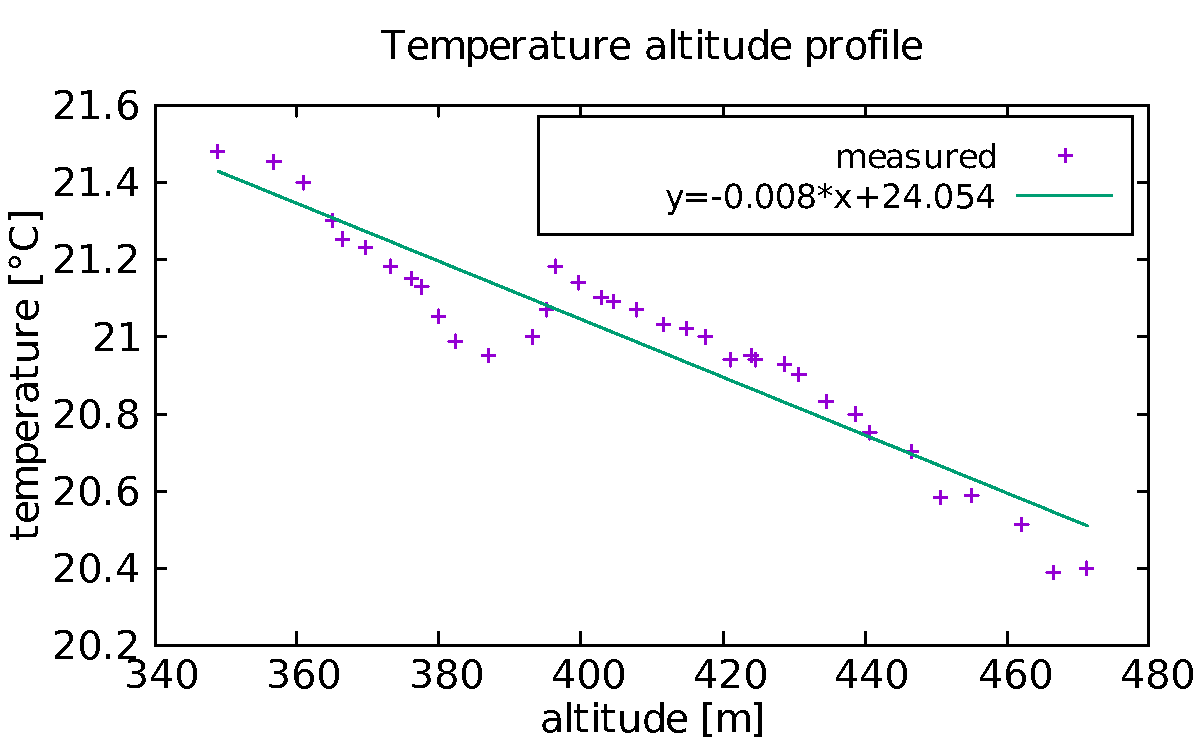
\includegraphics[width=250pt]{temp.pdf}
\label{temp2}
\end{figure}
\paragraph{Pressure.} The pressure measurements before launch were significantly deviated so they were removed from the data set. Even though pressure doesn't have a linear relationship (their real relationship is quazipolynomial close to an exponential converging to 0) the altitude difference during flight is low enough for linear relationship to be a close enough approximation, the result is shown in figure \ref{press}.
\begin{figure}[!h]
\centering
\caption{Non-deviating data-points of measured pressure}
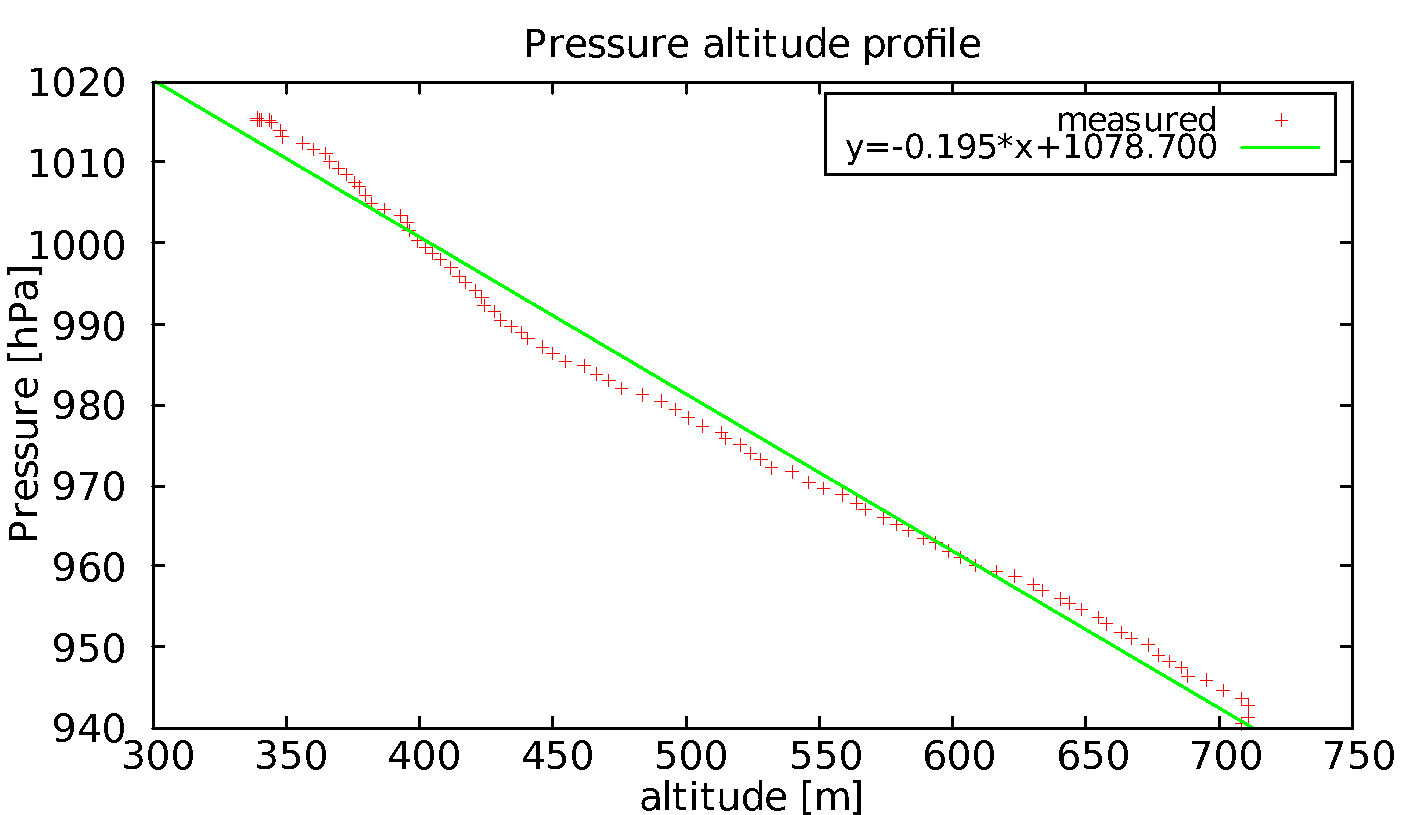
\includegraphics[width=250pt]{press.pdf}
\label{press}
\end{figure}
\paragraph{Humidity.} As relative humidity heavily depends on temperature it is better to plot absolute humidity. The problem is that the air in the cavity of the humidity sensor can have a slightly different temperature than the one in the temperature sensor. Even if they are a part of the same chip the air might not be as heated by the sun as the chip is. This causes the upward drift by both ends of figure \ref{hum1}. These values are removed in figure \ref{hum2}. That should provide a much more accurate measurement.
\begin{figure}[!h]
\centering
\caption{All data-points of absolute humidity}
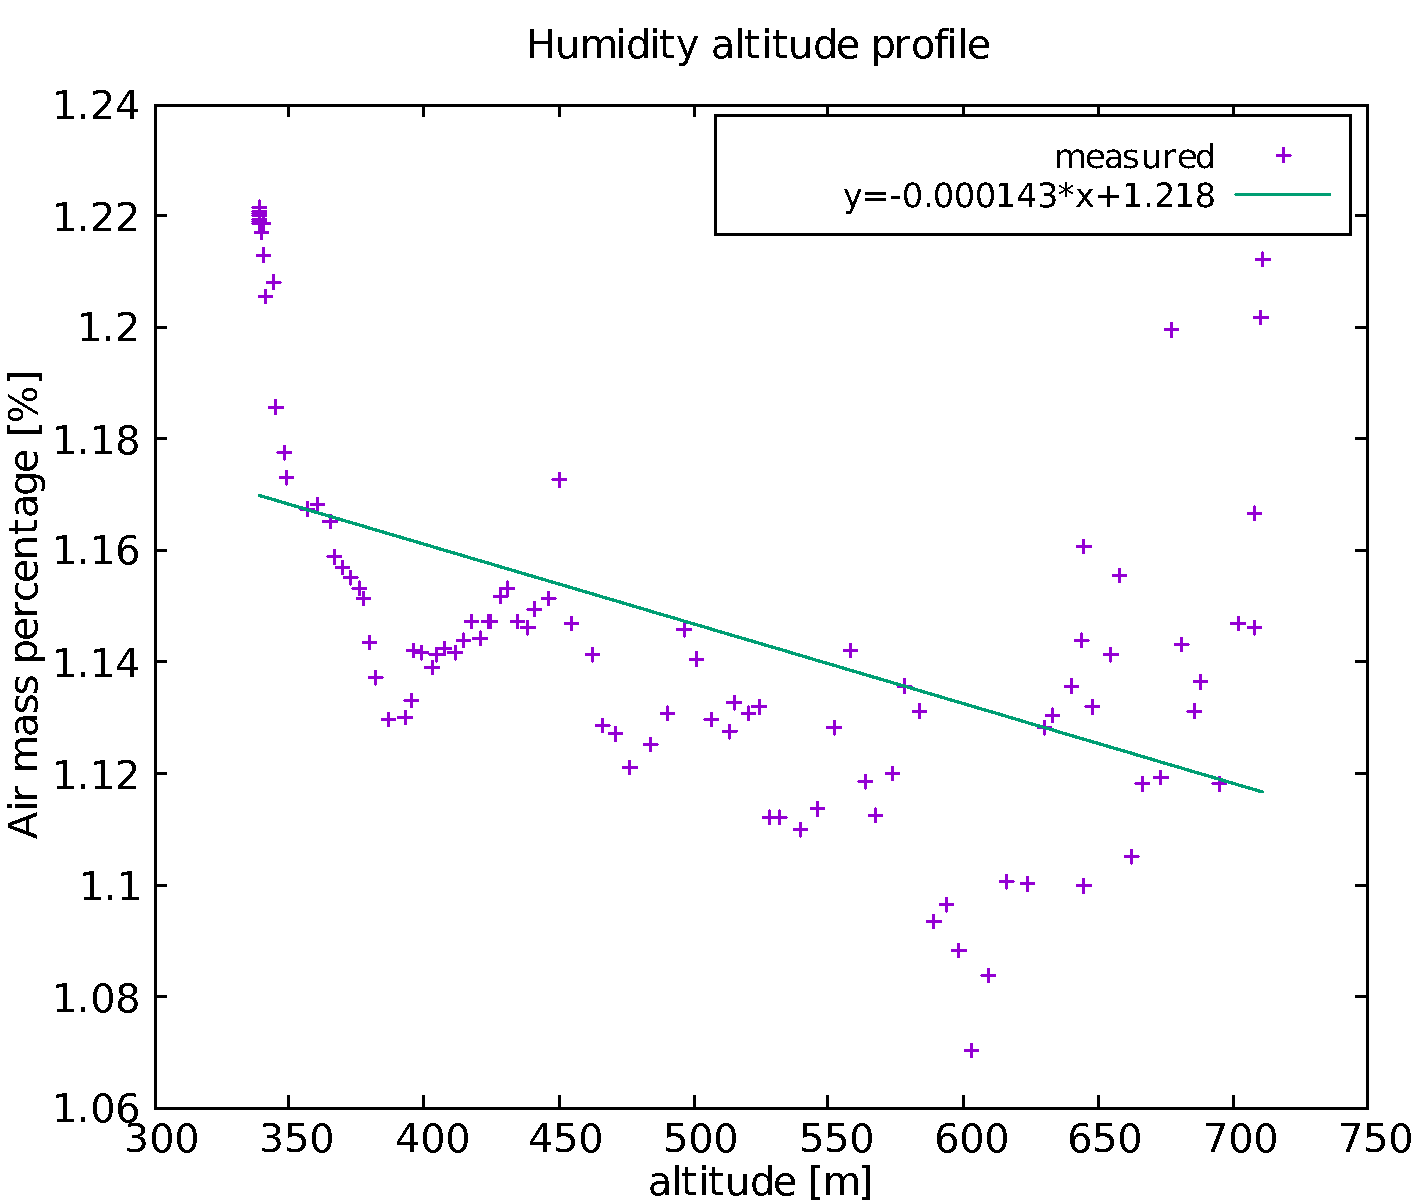
\includegraphics[width=250pt]{hum.pdf}
\label{hum1}
\end{figure}
\begin{figure}[!h]
\centering
\caption{Non-deviating data-points of absolute humidity}
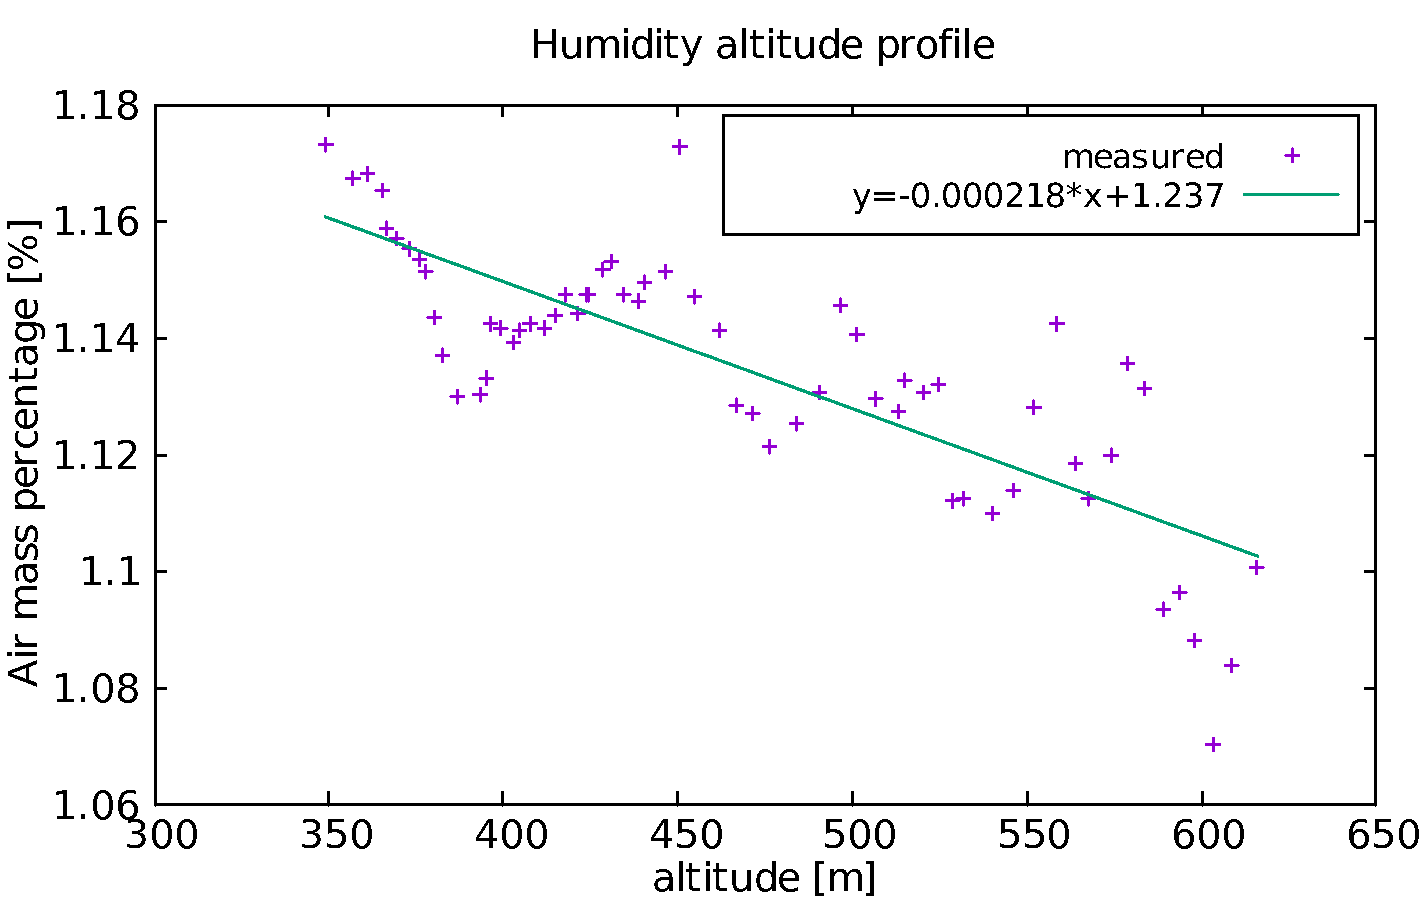
\includegraphics[width=250pt]{hum2.pdf}
\label{hum2}
\end{figure}
\subsubsection{Numeric results before atmospheric analysis}
Some are directly measured, some are calculated, some are sea-level values for linear variables, with earth reference values in the right column where reasonable, $latm$ is local atmospheric pressure, therefore partial pressure in $latm$ is equivalent to the portion of mass of that compound in comparison to the mass of air:\\
\begin{align}
p_0 &= (1078\rpm10)hPa & p_0 &= 1013.25hPa \cite{pressx}\\
T_0 &= (24.1\rpm2.1)\degree C & T_0 &= 22.7\degree C \cite{tempx}\\
\Delta T_{100m} &= (0.8\rpm0.1)\degree C & \Delta T_{100m} &= 0.66\degree C\\
AH &= (1.237\rpm0.024)\% latm & & \\
g &= (9.31\rpm0.66)ms^{-2} & g_{ref} &= 9.81ms^{-2}\\
\rho_{air} &= (2.09\rpm0.14)kgm^{-3} & \rho_{ref} &= 1.23kgm^{-3}\\
\Phi_B &= (38.8\rpm5.4)\mu T & \rho_{ref} &= 44.0\mu T\\
h_{atmosphere} &= (133 \rpm 10) km & &\\
p_{O_2} &= (20\rpm2) \% latm & p_{O_2ref} &= 20.89 \% latm \cite{lastx}\\
p_{CO_2} &= (0.6\rpm0.1) \% latm & p_{CO_2ref} &= 0.5 \% latm\\
p_{O_3} &= (35\rpm 5) ppb & & \\
T_{ground\_average} &= (17\rpm5)\degree C &  T_{ground_ref}\ &= 15 \degree C \cite{Jacob}\\
Em_{2} &= (5.9\rpm1.5) MJ & & \\
f &= (0.81\rpm0.05) & f_{ref} &= 0,77\cite{Jacob}
\end{align}
We can see that magnetic field is bigger than necessary.
\subsubsection{Atmospheric gas concentrations}
After fitting concentrations of gases and the amount of clouds\footnote{Cross sections for calculated gases were taken from \cite{cross1}, \cite{cross2}, \cite{cross3}, \cite{cross4}}, we obtain a fit seen in figure \ref{spectrome}. As the precision of the measurements isn't very high some gas concentrations could be significantly different. The biggest problem is that some gasses are invisible at all frequencies (of those only noble gases with the exception of Argon are stable in an oxygen rich environment). Another group of gasses that cause Rayleigh scattering ($O_2$, $N_2$, $Ar$) and $NO_2$ which has an absorption curve very similar to Rayleigh scattering curve. $NO_2$, $NO$, $O_2$ and $NO$ have equilibrium reactions induced by sunlight \cite{no2o3}, because ozone and oxygen concentration measured are both lower than average value on Earth and $NO$ isn't a stable molecule, $NO_2$ must also have a lower concentration than on Earth. Therefore effects of $NO_2$ are negligible. With that in mind the only possible fit would imply more than half of the atmosphere being made up of Xenon or even more of Argon. We are disregarding all unstable molecules that are not made by natural processes (e.g. volatile organic chemicals). Such high concentration of noble gasses is extremely unlikely in so high quantities as was explained in \ref{basic}, paragraph Atmospheric composition.\par
\begin{figure}[!h]
\centering
\caption{}
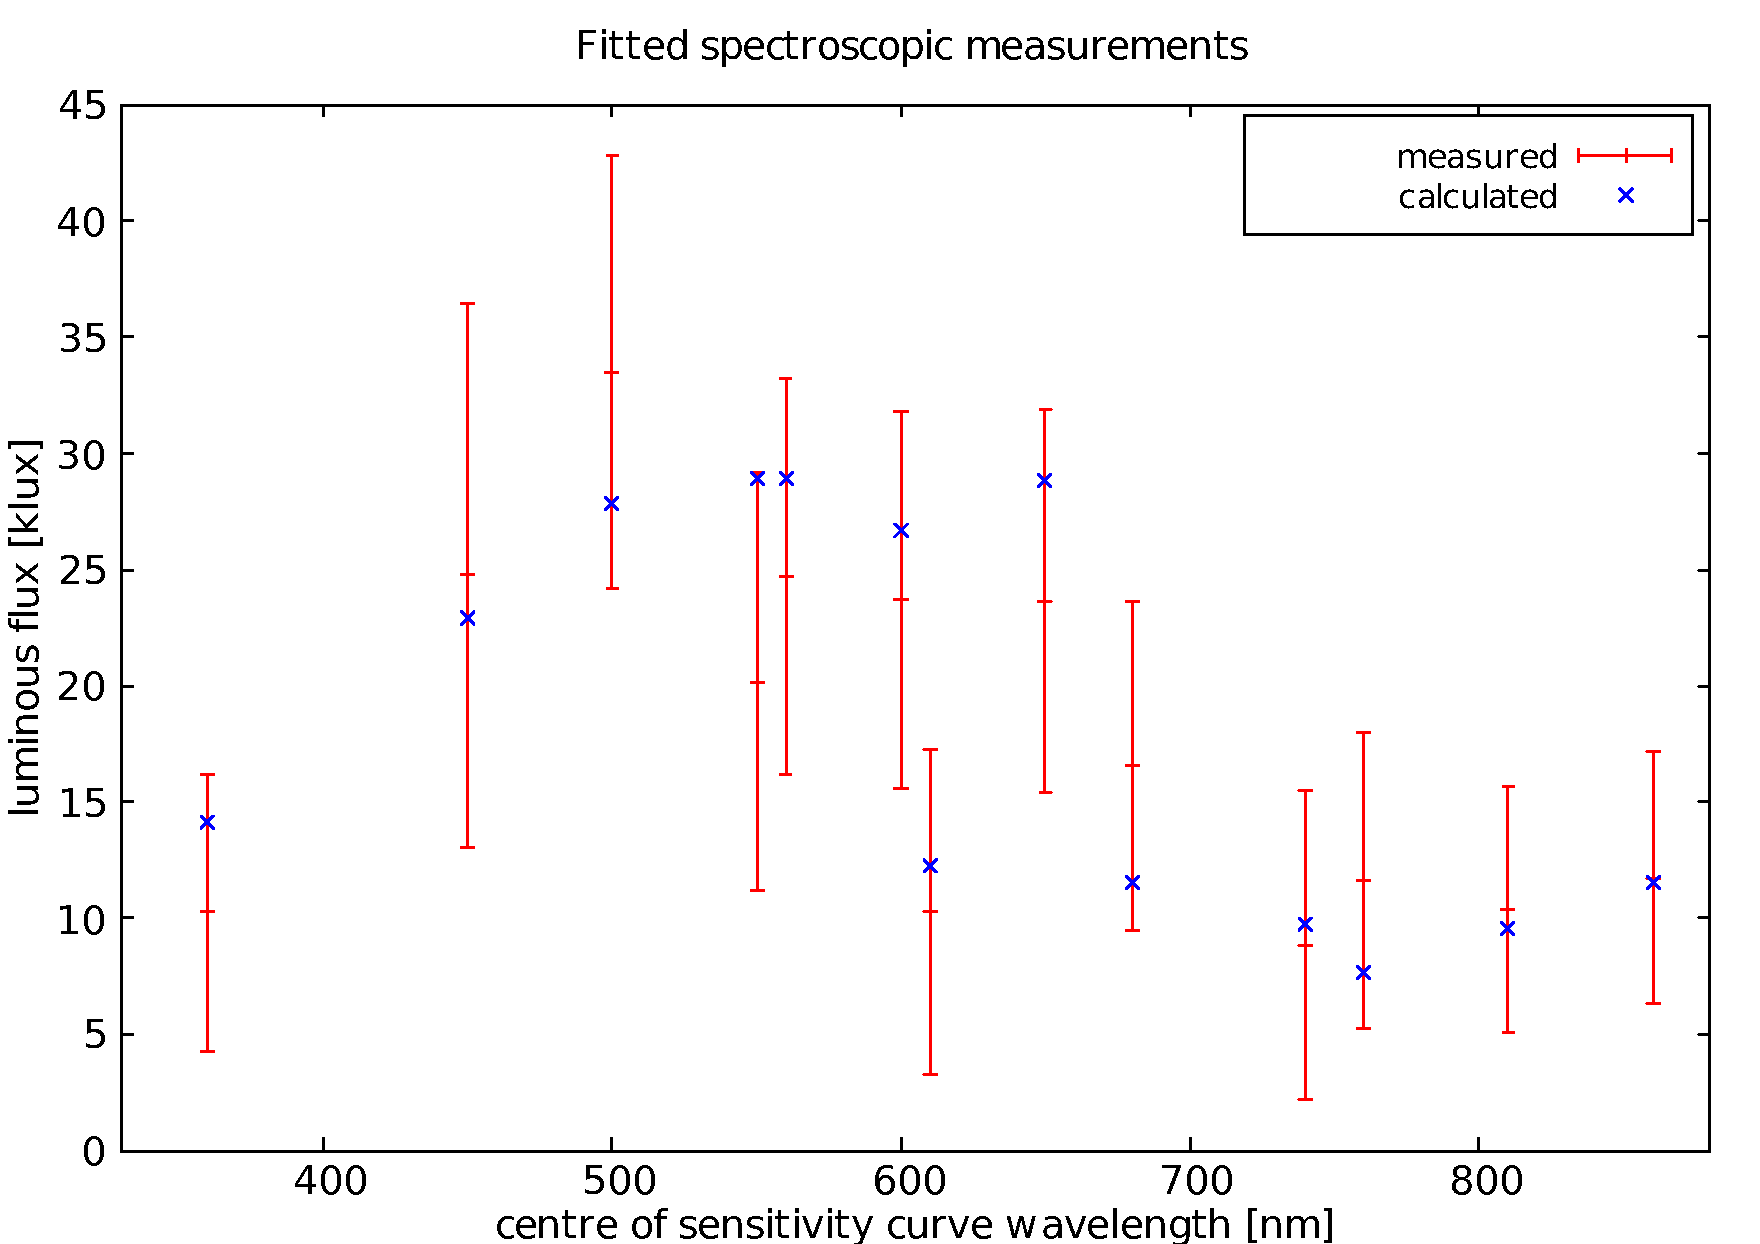
\includegraphics[width=250pt]{spectromeasure.pdf}
\label{spectrome}
\end{figure}
So we conclude that air density measurement is wrong and will only calculate with overall atmosphere mass, not the density. From this we get concentrations of gasses that affect the incoming radiation, reference values on the right:\\
\begin{align}
p_{N_2} &= (79\rpm10) \% latm & p_{N_2ref} &= 78.08 \% latm \cite{lastx}\\
p_{H_2O} &= (0.4\rpm0.2) \% latm & p_{O_2ref} &= 28.08 \% latm\\
p_{O_3} &= (1.4\rpm0.2) 10^{-4} \% latm & p_{O_2ref} &= 0.5 10^{-4} \% latm
\end{align}
We cannot be sure whether part of the nitrogen isn't Argon because they behave the same way spectrocopically and have nearly the same molecule mass. Ozone and water concentrations change a lot with height so it is correct that the value is different form the one at ground level. This is an average over the whole atmosphere. There is also a cloud cover or a large amount of particles in the air (aerosol or dust). How the result is influencing the light received on earth is in figure \ref{spectrocal}, partial effects on it in Appendix 1.
\begin{figure}[!h]
\centering
\caption{Recieved power at different wavelengths outside atmosphere, on a sunny day and on a slightly cloudy day as was when we measured}
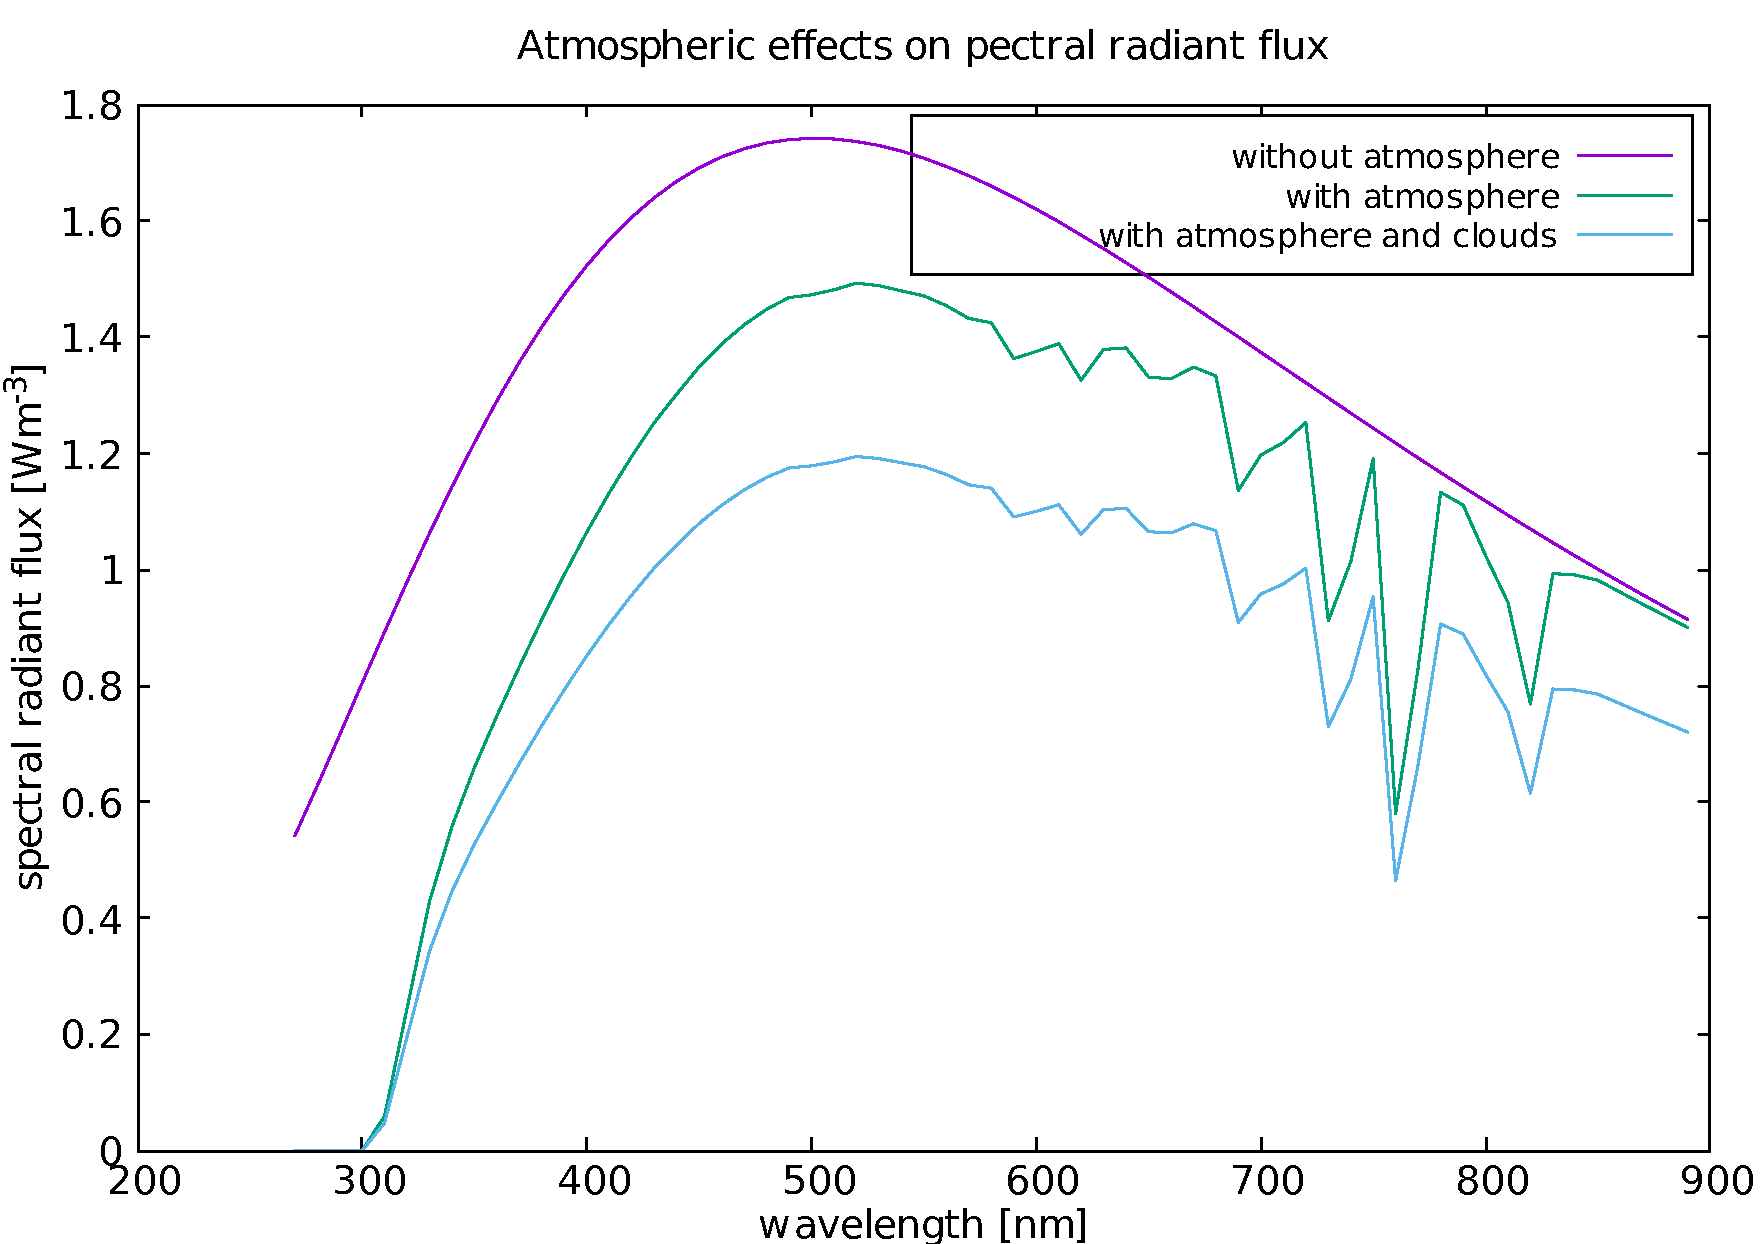
\includegraphics[width=250pt]{spectrocal.pdf}
\label{spectrocal}
\end{figure}
\paragraph{Greenhouse effect.} When we apply the greenhouse calculations on these results into greenhouse effect calculations, we get that no other greenhouse gasses are necessary for the desired effect. Because water level in the air is influenced by temperature, figure \ref{gr2} doesn't contain it and contains only the driving greenhouse gasses.
\begin{figure}[!h]
\centering
\caption{All greenhouse gasses}
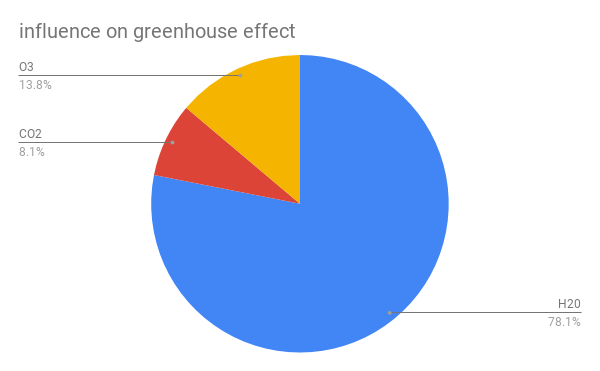
\includegraphics[width=250pt]{gr1.png}
\label{gr1}
\end{figure}
\begin{figure}[!h]
\centering
\caption{Driving greenhouse gasses}
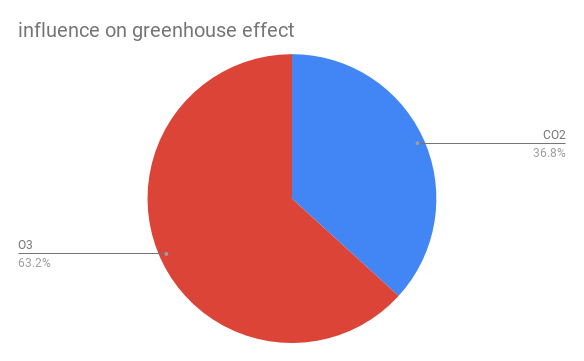
\includegraphics[width=250pt]{gr2.png}
\label{gr2}
\end{figure}
\section{Biological experiments}
\subsection{Methods}
\par
The CanSat had an sticky flycatcher attached to its side. An excavator took a sample of soil after landing. After the satellite was recovered, it was locked into an airtight metal box. It was opened in an airtight chamber which we constructed.
\par
The chamber for the biological experiments is airtight yet openable. During the first use and after each opening, it is sufficient to have samples isolated in a metal box and to irradiate the chamber for a few minutes with an internal UVC fluorescent lamp. \cite{Allen}
\begin{figure}[!h]
\centering
\caption{UVC mutation mechanism taken from \cite{Allen}}
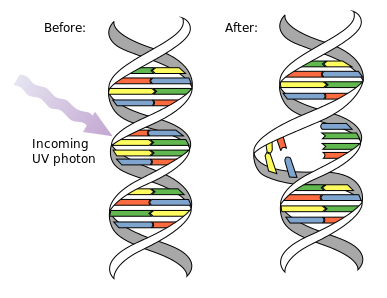
\includegraphics[width=230pt]{UVCmutation.png}
\end{figure}
The radiation of wavelength of 253.7 nm destroys the nuclei of the cells of all living organisms. UV light of a lower wavelength than 345 nm does not pass through the acrylic, so it is ideal to use acrylic for the shielding as well as it is transparent. \cite{Eplastics} At the same time, the UVC lamp generates lethal ozone, which is then removed by freon. 
\begin{align}
O_2 &\xrightarrow{\text{UVC}} O + O \\
O_2 + O &\xrightarrow{\text{UVC}} O_3
\end{align}
\par
We used Freon named "22", which is actually chlorodifluoromethane ($CHClF_2$). Ozone degradation works by a series of reactions. We assume that there were the following reactions between Freon 22 and ozone:\\
\begin{align}
Cl + O_3 &\xrightarrow{} ClO + O_2 \\
ClO + O &\xrightarrow{} Cl + O_2
\end{align}
\par And
\begin{equation}
O_3 + 2_H^+ + 2e^- \xrightarrow{} O_2 + H_2O
\end{equation}
\par After decontaminating and neutralising whole chamber and all equipment inside, it is possible to remove the samples from the box and work with them. The chamber also includes a heater, a water dispenser, a lighting and a fan. Using these devices, ideal cultivation conditions can be achieved, which boosts the growth of the bacteria. The normal cultivation time is 48 hours, which we did not have in the finals, but with the help of all the upgrades we managed to grow some samples. Sample identification was achieved with the help of an integrated microscope with internal motion. This invention allowed us to still plug the eyepiece into the wall, but it lead to the oscillation of the setup, thus worsening the observation conditions. All interior equipment was handled through wall-mounted gloves.
\begin{figure}[!h]
\centering
\caption{UVC radiation source on}
\includegraphics[width=230pt]{UVCradiation.JPG}
\end{figure}
\par
Outside the chamber, three agar samples were mixed. We cleaned them with UVC and ozone with the rest of the chamber. Then, within the chamber, we selected samples from the satellite. There were pieces of soil, a blade of grass. Also, small bugs came out of the satellite, another proof of life on the planet. Then, we applied antibiotics (Amoxicilin) to one of the samples. During the night the samples grew and we regularly observed them with the microscope. Since the start of an agar preparation phase, a camera has taken a photo every 10 seconds to avoid the manipulation with the samples.\footnote{The date and time were set incorrectly, but the chronological record ran correctly.}
\begin{figure}[!h]
\centering
\caption{Preparation of the agar}
\includegraphics[width=230pt]{Agarpreparation.JPG}
\end{figure}
\par The basic analysis of the sample was the Gram method; one of the basic procedures in microbiology. Gram staining identified the bacteria as either Gram positive (G+) and Gram negative (G-). This division is based on a different structure of the bacterial wall. The samples were taken from the chamber around 6:30 local time. It left us only 2.5 hours until the final presentation. In such a short time it was not possible to visibly grow colonies that would not come from the original sample.
\begin{enumerate}
  \item The selected sample was transferred to the slide. This sample was put into the flame of the candle for a few seconds. The sample temperature could not exceed 80 degrees Celsius.
  \item Crystal violet was applied to the preparation for two minutes.
  \item Subsequently, it was necessary to turn violet and apply Gram's reagent to the sample, which is an aqueous solution of potassium iodide and crystalline iodine at a concentration of 2 to 1. Then, we waited until the whole sample turned black.
  \item We washed the sample with 96\% ethanol until the reagent flowed out of the sample.
  \item We carefully rinse the sample with water for about two minutes.
  \item The last staining was done with safranin, lasting for as long as five minutes.
  \item Again, we washed the dye with water. Then, we dried the sample. Gram method was finished.
\end{enumerate}
\begin{figure}[!h]
\centering
\caption{Gram staining taken from \cite{Labfo}}
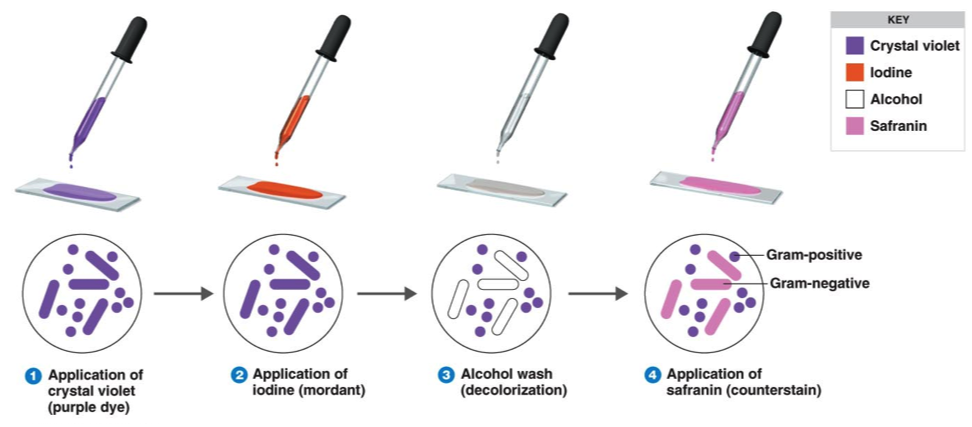
\includegraphics[width=230pt]{Gramprocedure.png}
\end{figure}
\subsection{Results}
\par
Based on our experience from previous microscopy tests, we were able tu identify the group of Actinomycete belonging to gram-positive bacteria in the sample. Conversely, no gram-negative bacteria were identified. These results are in line with our assumptions. Gram-positive bacteria show the existence of life on the surface. On the other hand, negative analysis of gram-negative bacteria is also expectable. Gram-negative bacteria usually belong to dangerous pathogens, which are not to be expected in soil or air. Their presence would point to external contamination, which did not happen.
\par
As was mentioned in part above, several beetles and a blade of grass were trapped by the sticky insect trap. Therefore, it is possible to consider a very diverse life on the surface of the planet under investigation.
\par
In total, we created four samples. First of them was the specimen where we covered the surface of the agar with antibiotics. Gram method did not show any signs of life, so it did not differ from the reference. Based on our observation we can assume that the antibiotics functioned correctly and this experiment was set up correctly. Sample number two included small, partially scattered colonies of Gram-positive bacteria, which corresponds to the fact that these colonies originate from atomised clay that was obtained from our Cansat.
\begin{figure}[!h]
\centering
\caption{Sample number two}
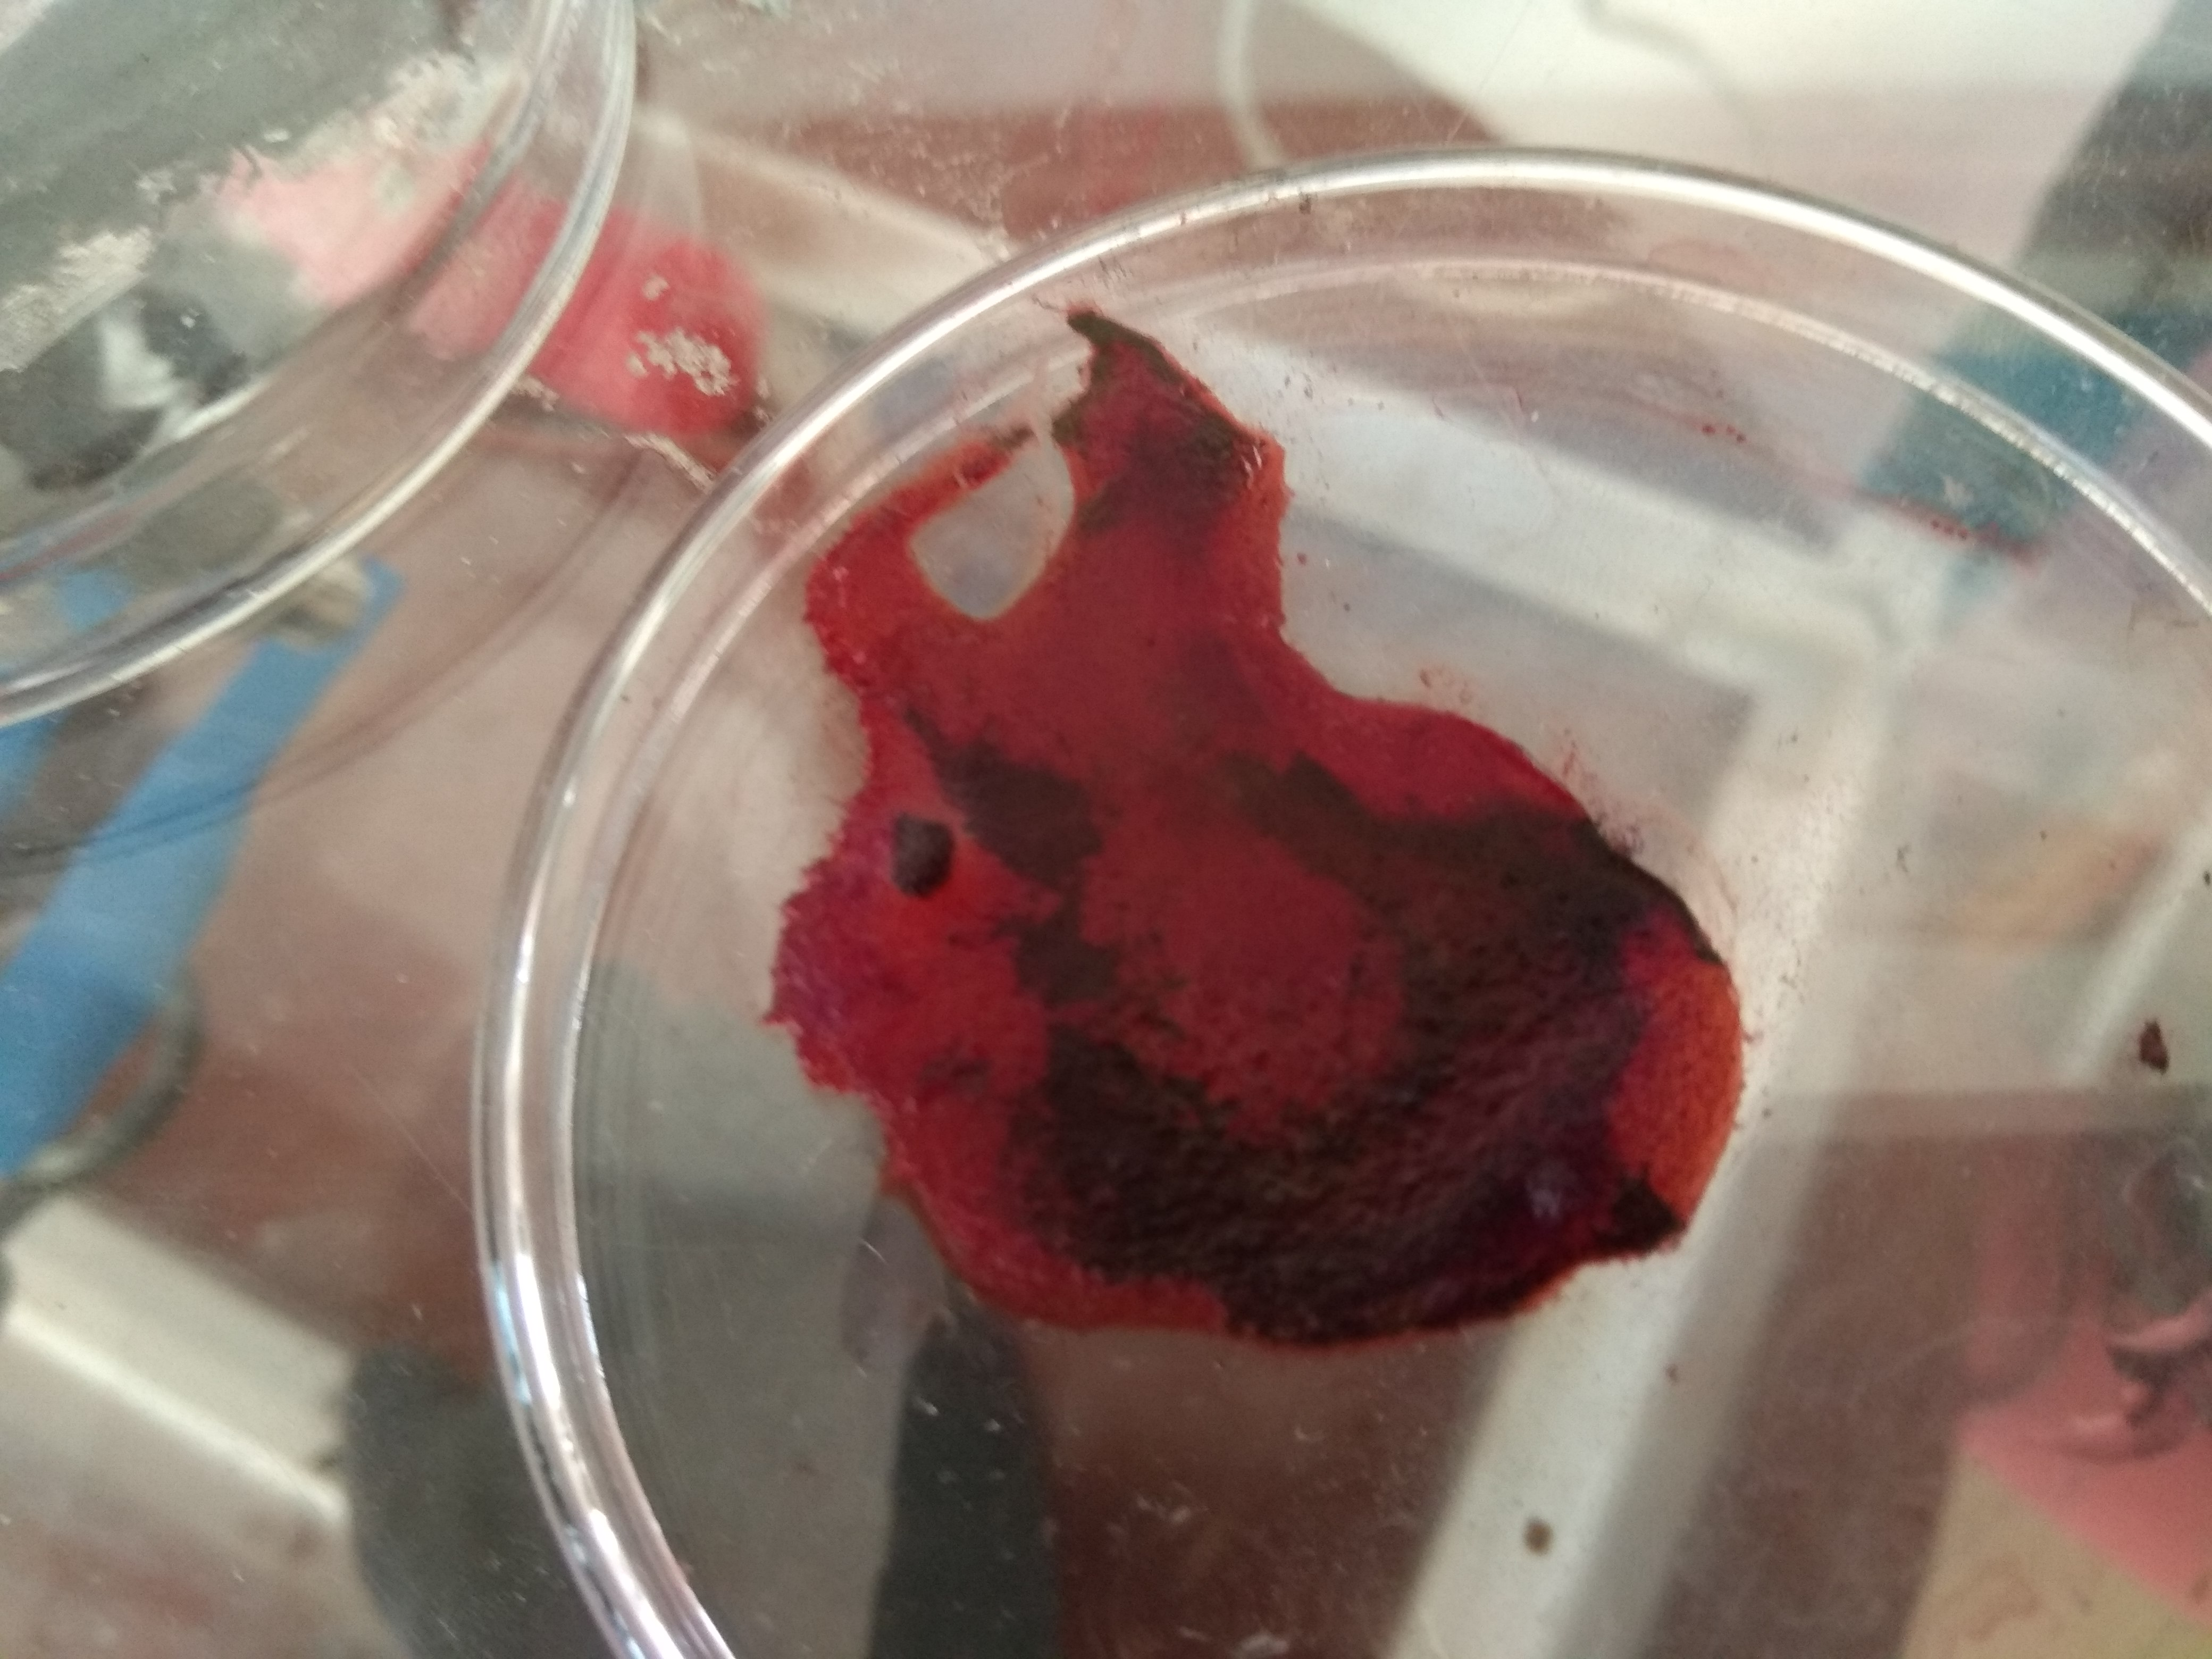
\includegraphics[width=230pt]{Sample-soil.jpg}
\end{figure}
\par
Sample number three shows a distinct colony of Gram-positive bacteria. The reason is that the sample contained a blade of grass containing various bacteria whose colonies grew around the stem.
\begin{figure}[!h]
\centering
\caption{Sample number three}
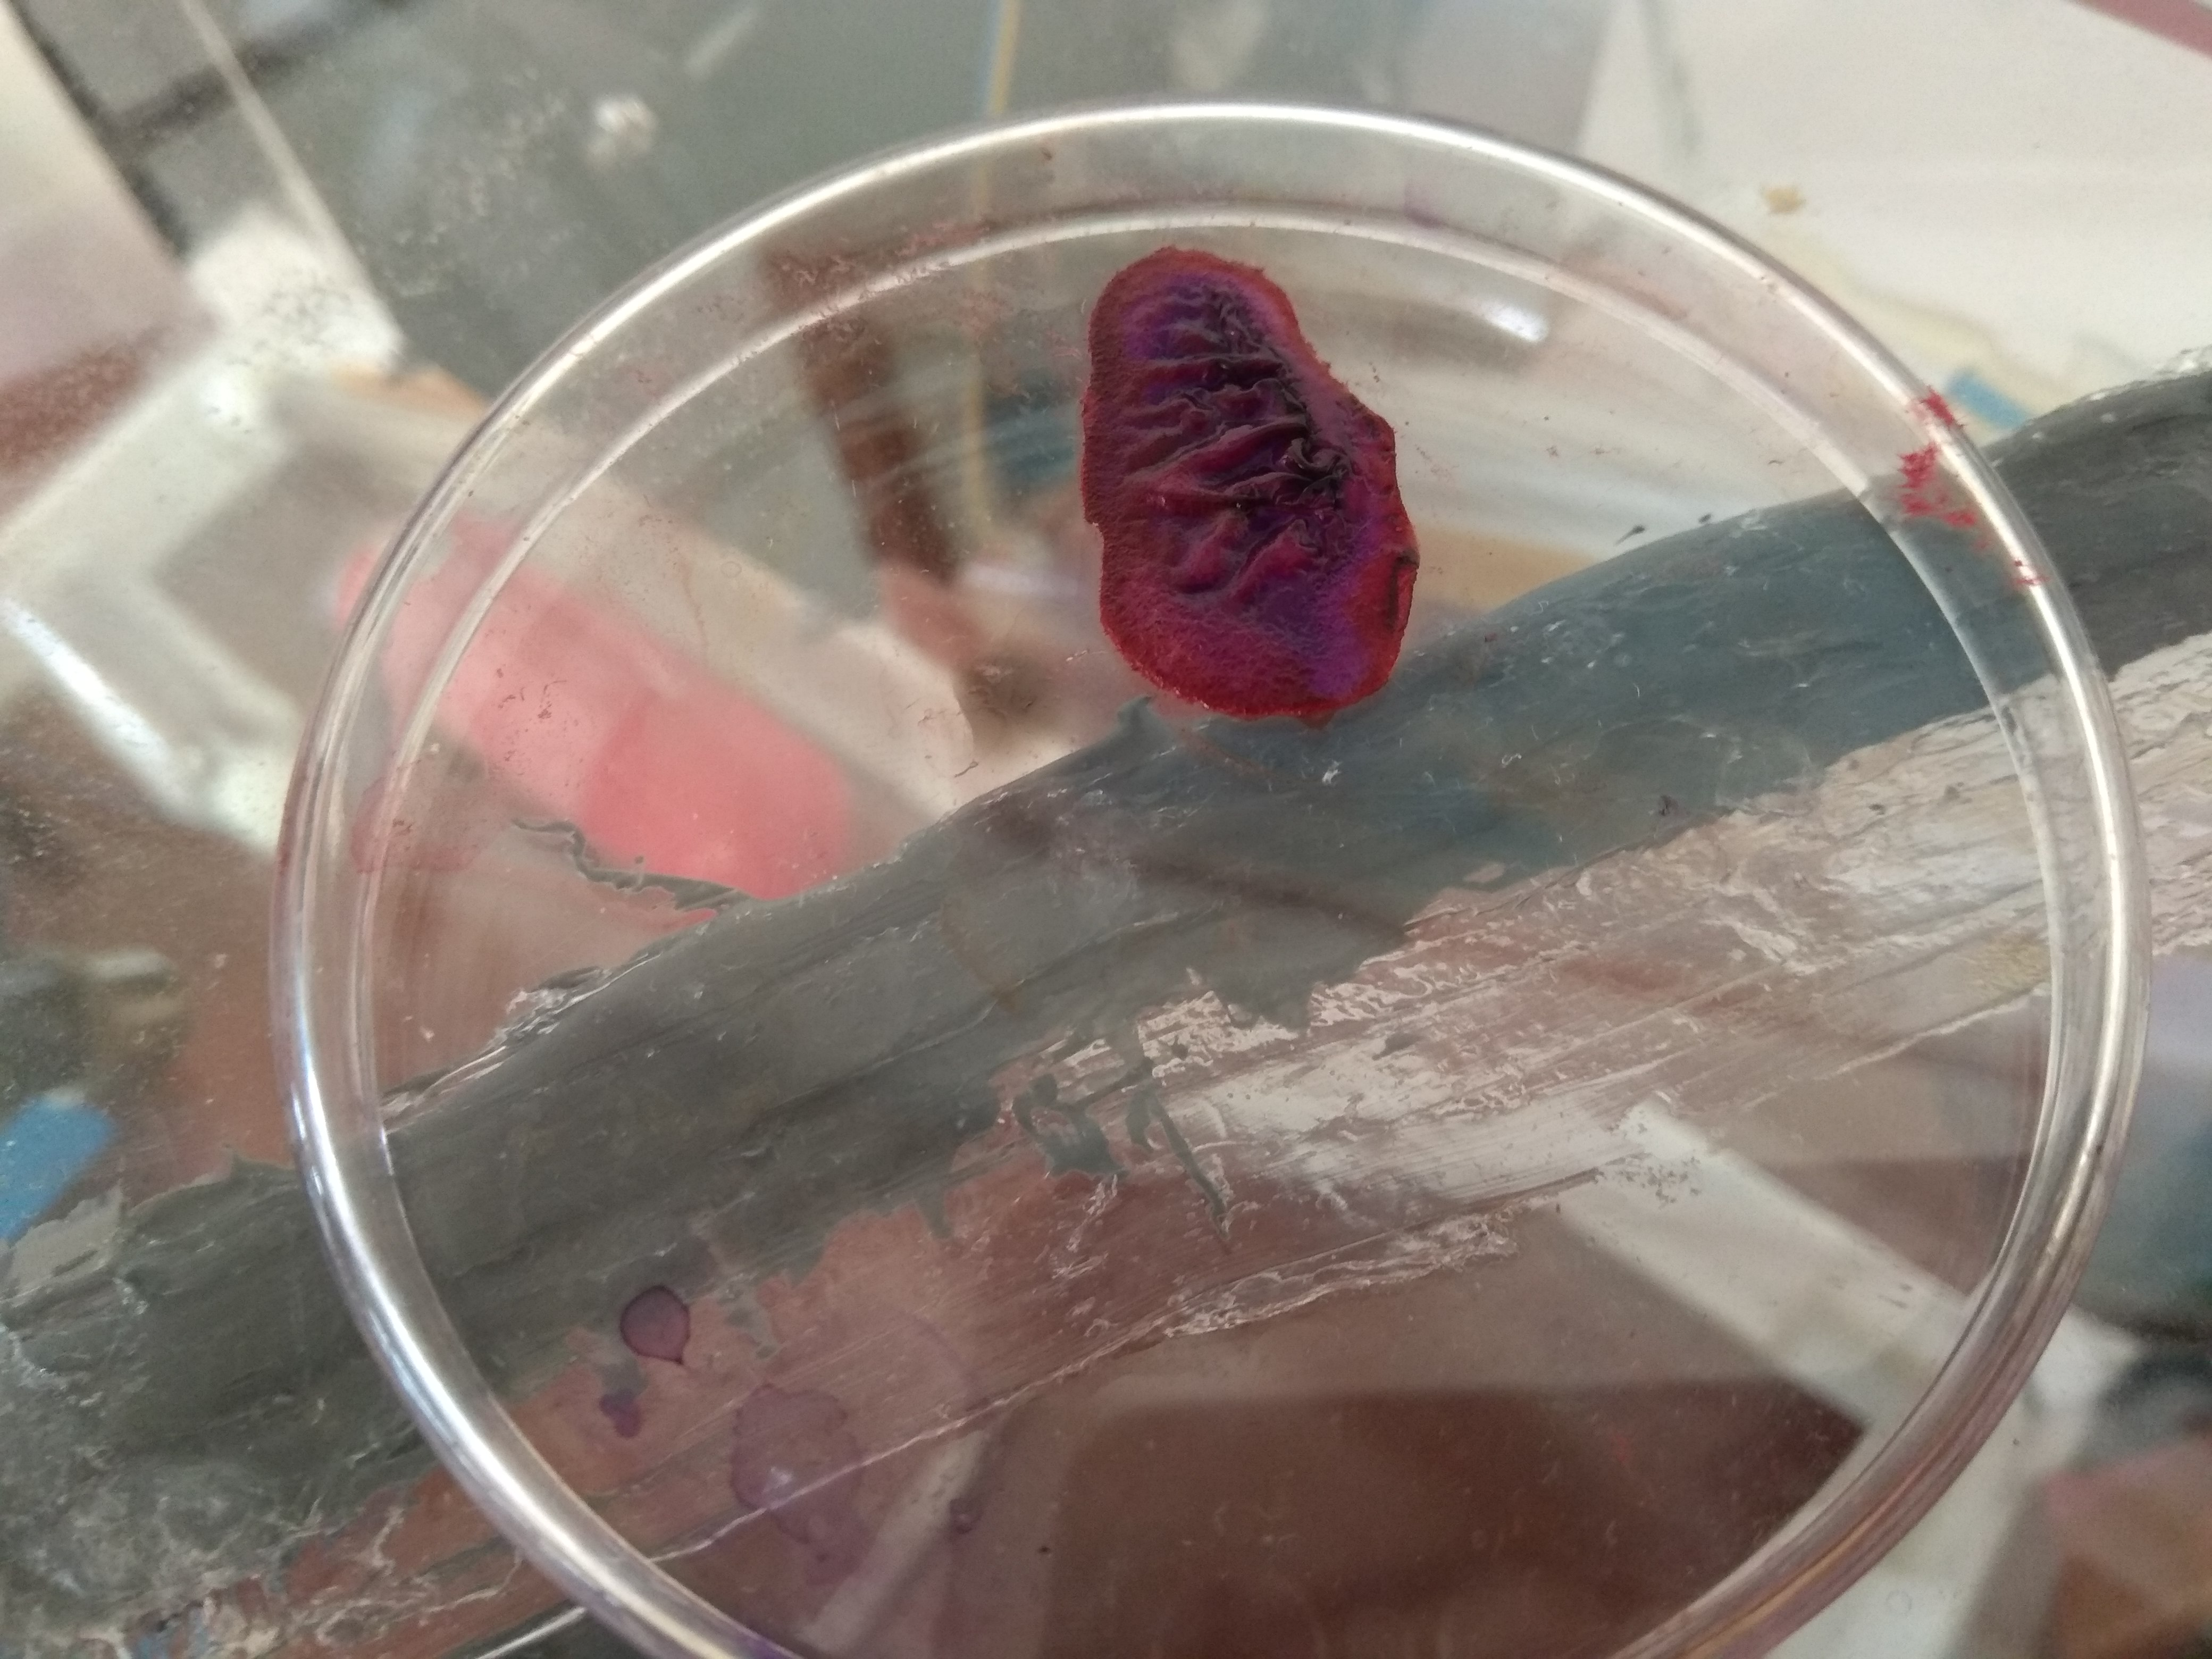
\includegraphics[width=230pt]{Sample-stem.jpg}
\end{figure}
\par
The last sample fully met our expectations because Gram staining was negative - in other words, there were neither Gram-positive nor Gram-negative bacteria. This sample was clear and should confirm that no samples were contaminated in the chamber or during staining.
\begin{figure}[!h]
\centering
\caption{Reference sample}
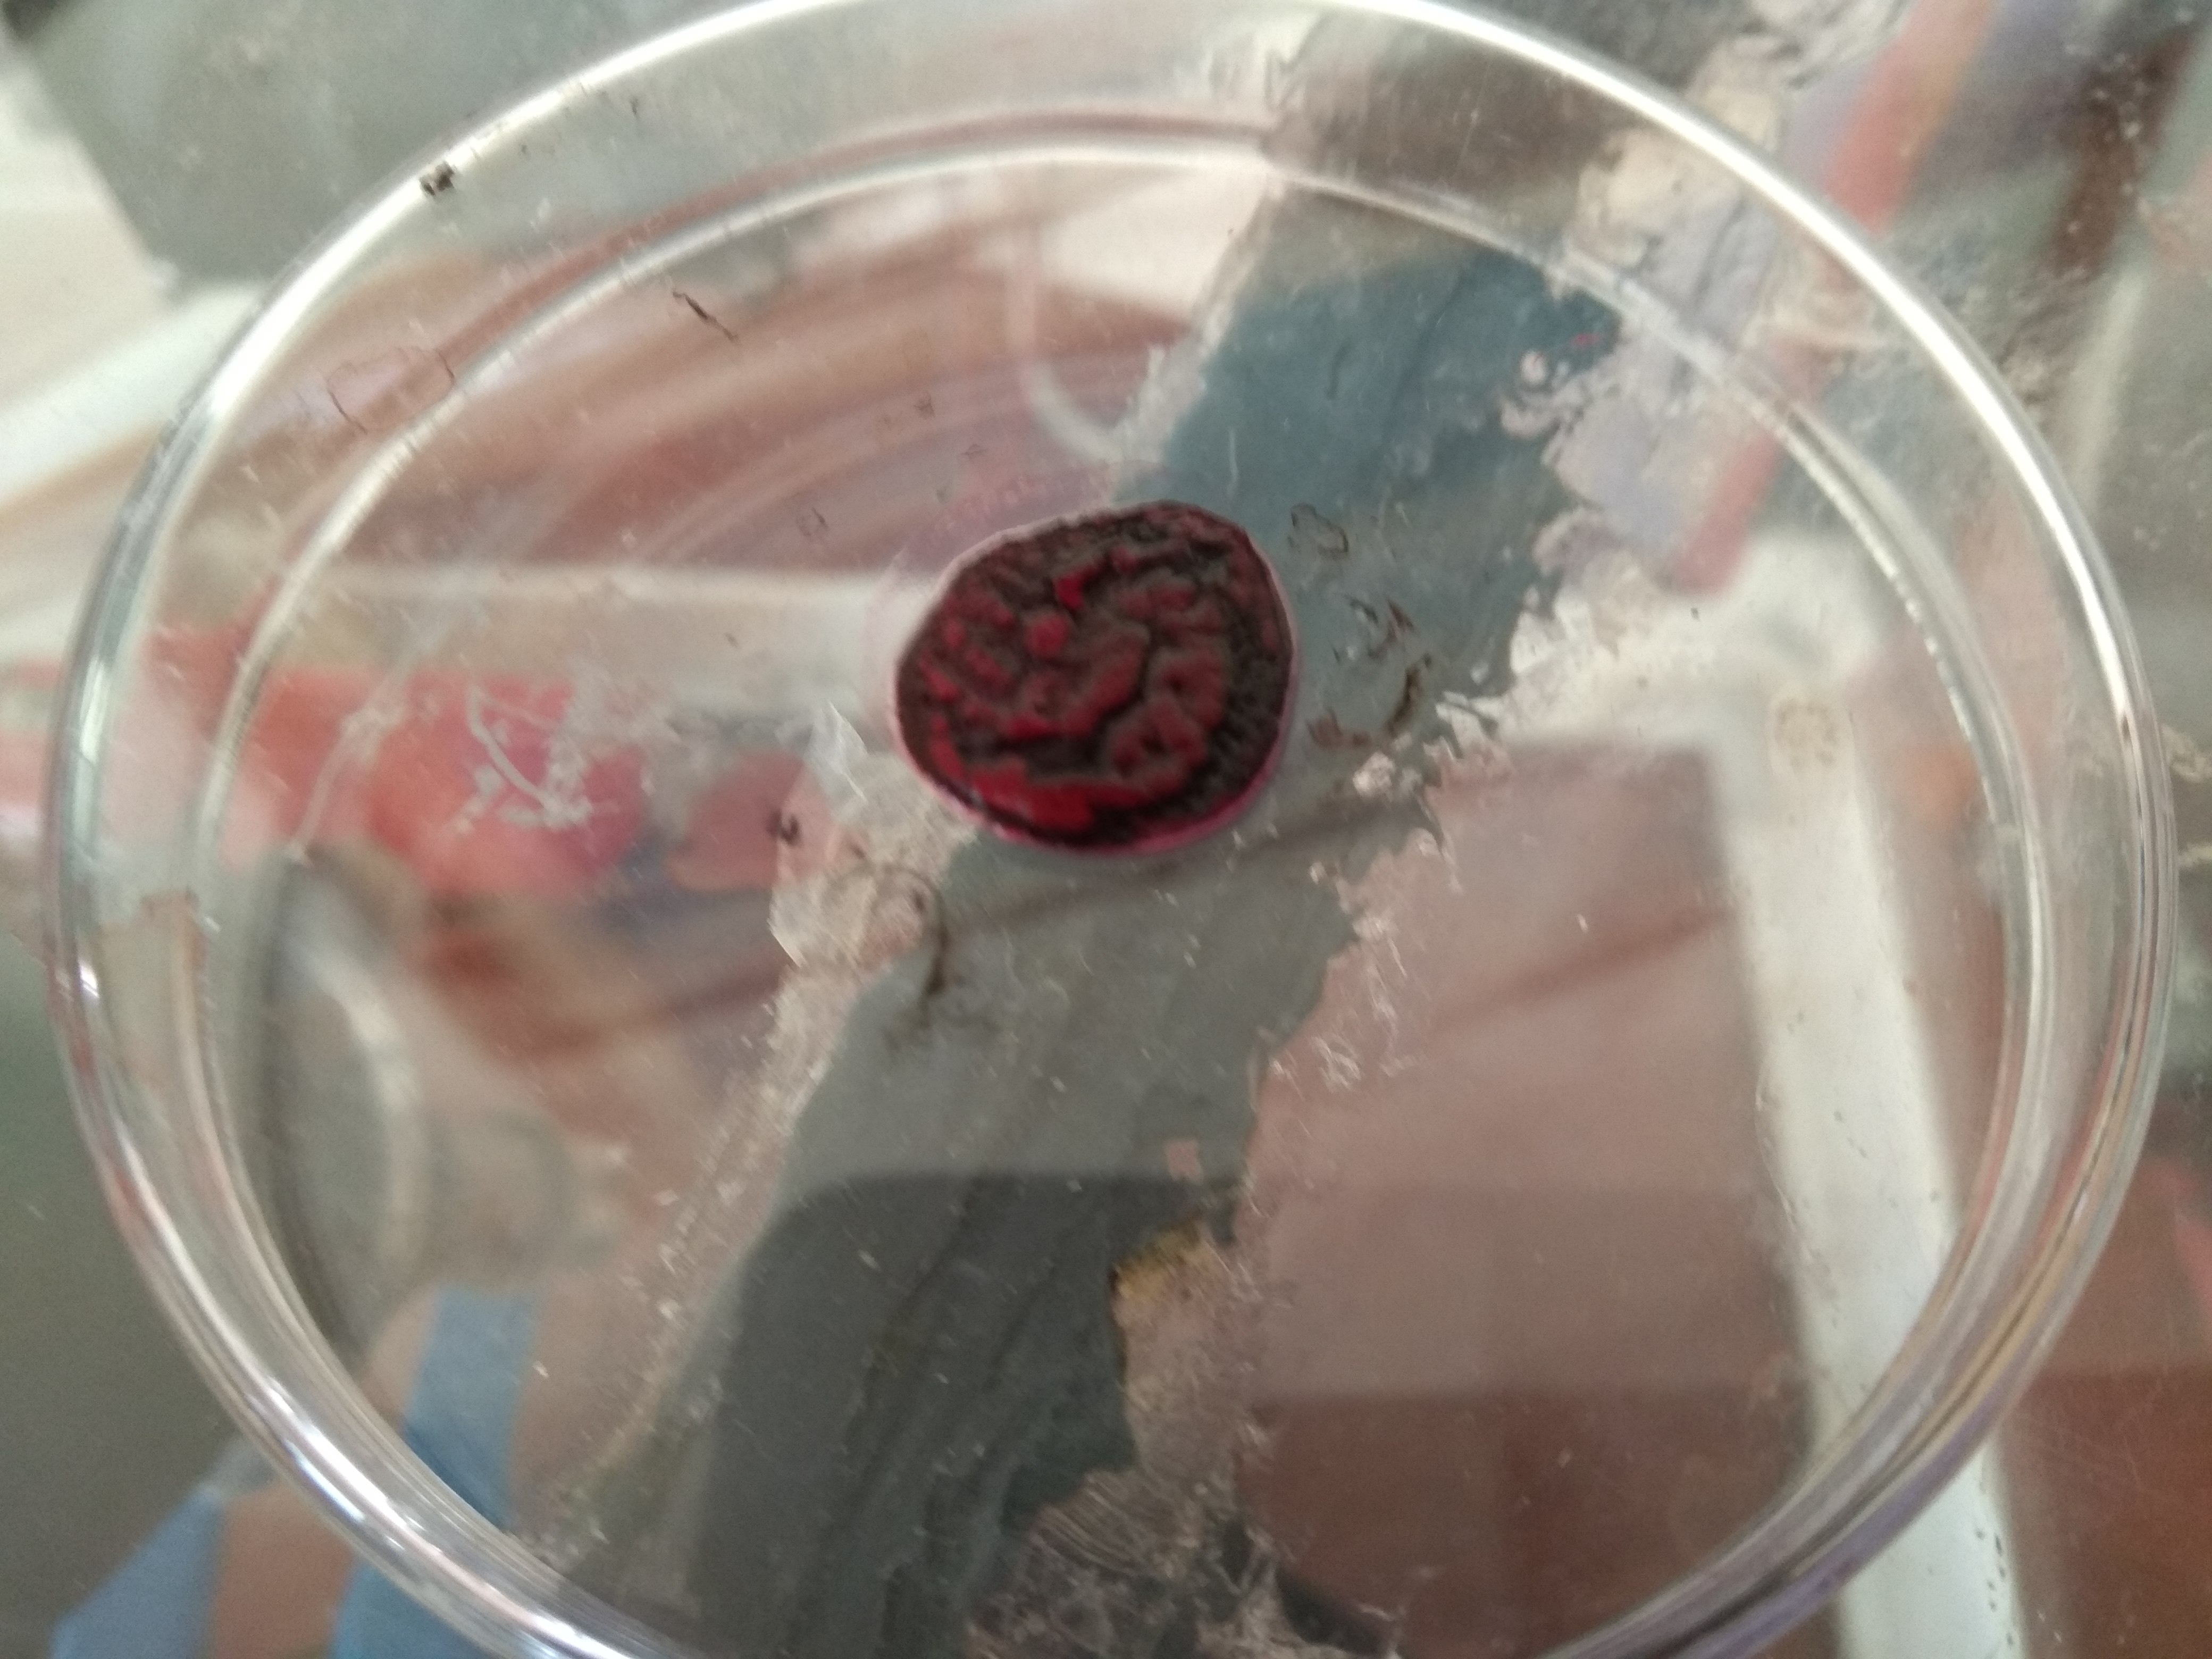
\includegraphics[width=230pt]{Reference_sample.jpg}
\end{figure}
\section{Discussion}
\subsection{Biological experiments}
\par
Referring to the results (especially to the negative reference sample), it can be argued that our method of chamber cleaning and sample isolation was conclusive. Gram-negative or Gram-positive bacteria could not be introduced. It should be noted that there is also a group of gram-neutral bacteria that do not interact with a given colouring method. Their occurrence was not detected, but it was not even announced. It is most likely that our samples handling is fully valid.
\subsection{Basic variables}
The biggest problem is with the slope in pressure measurements. It should be much smaller and it propagates into unusual air density. It is possible that it was caused by a leak of some unusual gasses (for example Xenon as suggested in results or some heavy organic gas) but that is quite unlikely but if it were true (if supported by other measurements) it would signify either volcanic or industrial activity. Another possibility is a drift (a change over time) either induced by climate or by sensor fault but the change stops when the CanSat reaches ground so that is ruled out. Last possibility is sensor fault. Other variables came within error margin of the reference value so that is ok.
\subsection{Spectroscopic measurements}
The level of precision of the measurements was quite low so it is impossible to take the results as certain. They are however the most likely results with the level of detail our model simulates. There is propably a relation with amount of UV from the star and overall ozone levels, but neither of us is a chemist so we didn't calculate such longtime equilibrium. The major problems with spectroscopy are exchangeable gases. We calculated corectly the sum of nitrogen and argon but their respective values.
\subsection{Greenhouse effect calculations}
This is an approximation of very complex phenomena. Not all of them have been explored yet, so the functionality of the model is limited to the troposphere. Then, all radiation from Earths surface is considered to be long-wave. Also the errors from spectroscopic analysis propagated here. This was especially the case fore ozone for which $7/4$ of standard value were calculated. This is possible on Earth but it happens extremely rarely. That caused ozone to be majority greenhouse gas even though it usually accounts for about one third. That in turn caused no need for other gasses, which on Earth exist.
\section{Conclusion}
We successfully proved all the necessary conditions for life to exist we could think of. The atmosphere is most likely nice and everything else is with near certainty. The only thing we didn't test directly was radioactivity but the life we found would unlikely have been there if there was an unreasonable amount of it. We found microscopic life - some bacteria - and macroscopic life - a plant and a bug. This is a final proof of habitability.
\begin{acknowledgements}
The project has also been assisted our teacher Mgr. Lenka Vinklerová, post-analysis has been assisted by Š. Karch,
\end{acknowledgements}
%-------------------------------------------------------------------

\begin{thebibliography}{}

%  \bibitem{baker} EXAMPLE: Baker, N. 1966,
%      in Stellar Evolution,
%      ed.\ R. F. Stein,\& A. G. W. Cameron
%      (Plenum, New York) 333
      
      
  \bibitem{Allen} \href{https://earthobservatory.nasa.gov/Features/UVB/}{NASA EO/Jeannie Allen - 	
Ultraviolet Radiation: How it Affects Life on Earth}

  \bibitem{Giesen} \href{http://www.jgiesen.de/astro/solarday.htm}{Giesen Juergen - How to compute the length of a day}
  
    \bibitem{Strobel}\href{http://www.astronomynotes.com/solarsys/s3c.htm} {Nick Strobel, Astronomynotes - Surface temperature}
    
    \bibitem{Geocraft}\href{http://www.geocraft.com/WVFossils/greenhouse_data.html} {Geocraft - Water Vapor Rules the Greenhouse System}


    \bibitem{TBZ}\href{https://stavba.tzb-info.cz/docu/tabulky/0000/000086_katalog.html}{TZB - Material properties catalogue}


    \bibitem{Jacob}\href{http://acmg.seas.harvard.edu/people/faculty/djj/book/bookchap7.html}{Daniel Jacob - Chapter 7 The Greenhouse Effect in Introduction to Atmospheric Chemistry}

\bibitem{Labfo}\href{https://laboratoryinfo.com/gram-staining-principle-procedure-interpretation-and-animation/} {LaboratoryInfo - Gram Staining : Principle, Procedure, Interpretation and Animation}

\bibitem{Eplastics}\href{http://www.eplastics.com/plexiglass_acrylic_sheet_uv_filter} {Eplastics - Plexiglass Acrylic Sheet - UV Filtering}

\bibitem{cross1} \href{http://www.wmo.int/pages/prog/arep/gaw/documents/FINAL\_GAW\_218.pdf}{WMO}
\bibitem{cross2} http://irina.eas.gatech.edu/EAS8803\_Fall2009/Lec6.pdf {Georgia Institute of Technology - Irina Sokolik}
\bibitem{cross3} \href{https://www.colorado.edu/chemistry/volkamer/publications/group-pubs/thalman-2014-rscsNArO2air-accepted.pdf}{Colorado University}
\bibitem{cross4} Orphal, J. "A critical review of the absorption cross-sections of O3 and NO2 in the ultraviolet and visible." Journal of Photochemistry and Photobiology A: Chemistry 157.2-3 (2003): 185-209.

\bibitem{Humidity} Lawrence, Mark G. "The relationship between relative humidity and the dewpoint temperature in moist air: A simple conversion and applications." Bulletin of the American Meteorological Society 86.2 (2005): 225-234.

\bibitem{no2o3} https://earthobservatory.nasa.gov/Features/ChemistrySunlight/chemistry\_sunlight3.php

\bibitem{Trenberth} Trenberth, K. E., and C. J. Guillemot, 1994: The total mass of the atmosphere. J. Geophys. Res., 99, 23079–23088.

\bibitem{Tinetti} Tinetti, G \& Encrenaz, Thérèse \& Coustenis, Athena. (2013). Spectroscopy of planetary atmospheres in our Galaxy. The Astronomy and Astrophysics Review. 21. 10.1007/s00159-013-0063-6. 

\bibitem{Fritz} Fritz, Sigmund, (1949). THE ALBEDO OF THE PLANET EARTH AND OF CLOUDS. Journal of Meteorology, 10.1175/1520-0469(1949)006<0277:TAOTPE>2.0.CO;2  

\bibitem{Bhattacharyya} Bhattacharyya, Tapas, (2015). The Soil: A Natural Resource. ISBN: 81-903797-7-1

\bibitem {Ozone co2e} Life Cycle Assessment Methodology Sufficient to Support Public Declarations and Claims, Committee Draft Standard, Version 2.1. Scientific Certification Systems, February 2011. Annex B, Section 4. %( Wiki - Ozone "48")
\bibitem {Git-Circuit}\href{github.com/suchanekj/CanSatGOSA/tree/master/CanSat2.0/Schematics/Circuit}{Github/../Circuit}

\bibitem {Git-Code}\href{https://github.com/suchanekj/CanSatGOSA/tree/master/CanSat2.0/Code} {Github/../Code}

\bibitem {Websites} \href{gosa.cz}{gosa.cz}

\bibitem{droplet radius} \href{https://www.atmos-chem-phys.net/7/3507/2007/acp-7-3507-2007.pdf}{atmos-chem-phys}

\bibitem{density of cloud} \href{https://water.usgs.gov/edu/watercycleatmosphere.html}{USGS}

\bibitem{refra} Sæmundsson, Þorsteinn (1986). "Astronomical Refraction". Sky and Telescope. 72

\bibitem{tempx} Joao Paulo Ii, Portugal History | Weather Underground. Weather Forecast & Reports - Long Range & Local | Weather Underground [online]. Copyright © Copyright TWC Product and Technology LLC 2014, 2018 [cit. 15 July 2018]. Website: https://www.wunderground.com/history/daily/LPPD/date/2018-6-26?req\_city=Ponta\%20Delgada&req\_statename=Portugal
\bibitem{pressx}International Civil Aviation Organization. Manual of the ICAO Standard Atmosphere, Doc 7488-CD, Third Edition, 1993. ISBN 92-9194-004-6.
\bibitem{lastx}Zimmer, Carl (3 October 2013). "Earth's Oxygen: A Mystery Easy to Take for Granted". New York Times. Retrieved 3 October 2013.

\end{thebibliography}
\newpage
\pagebreak
\clearpage
\section{Apendix 1}
\begin{figure}[!h]
\caption{Partial effects of different compounds of the atmosphere}
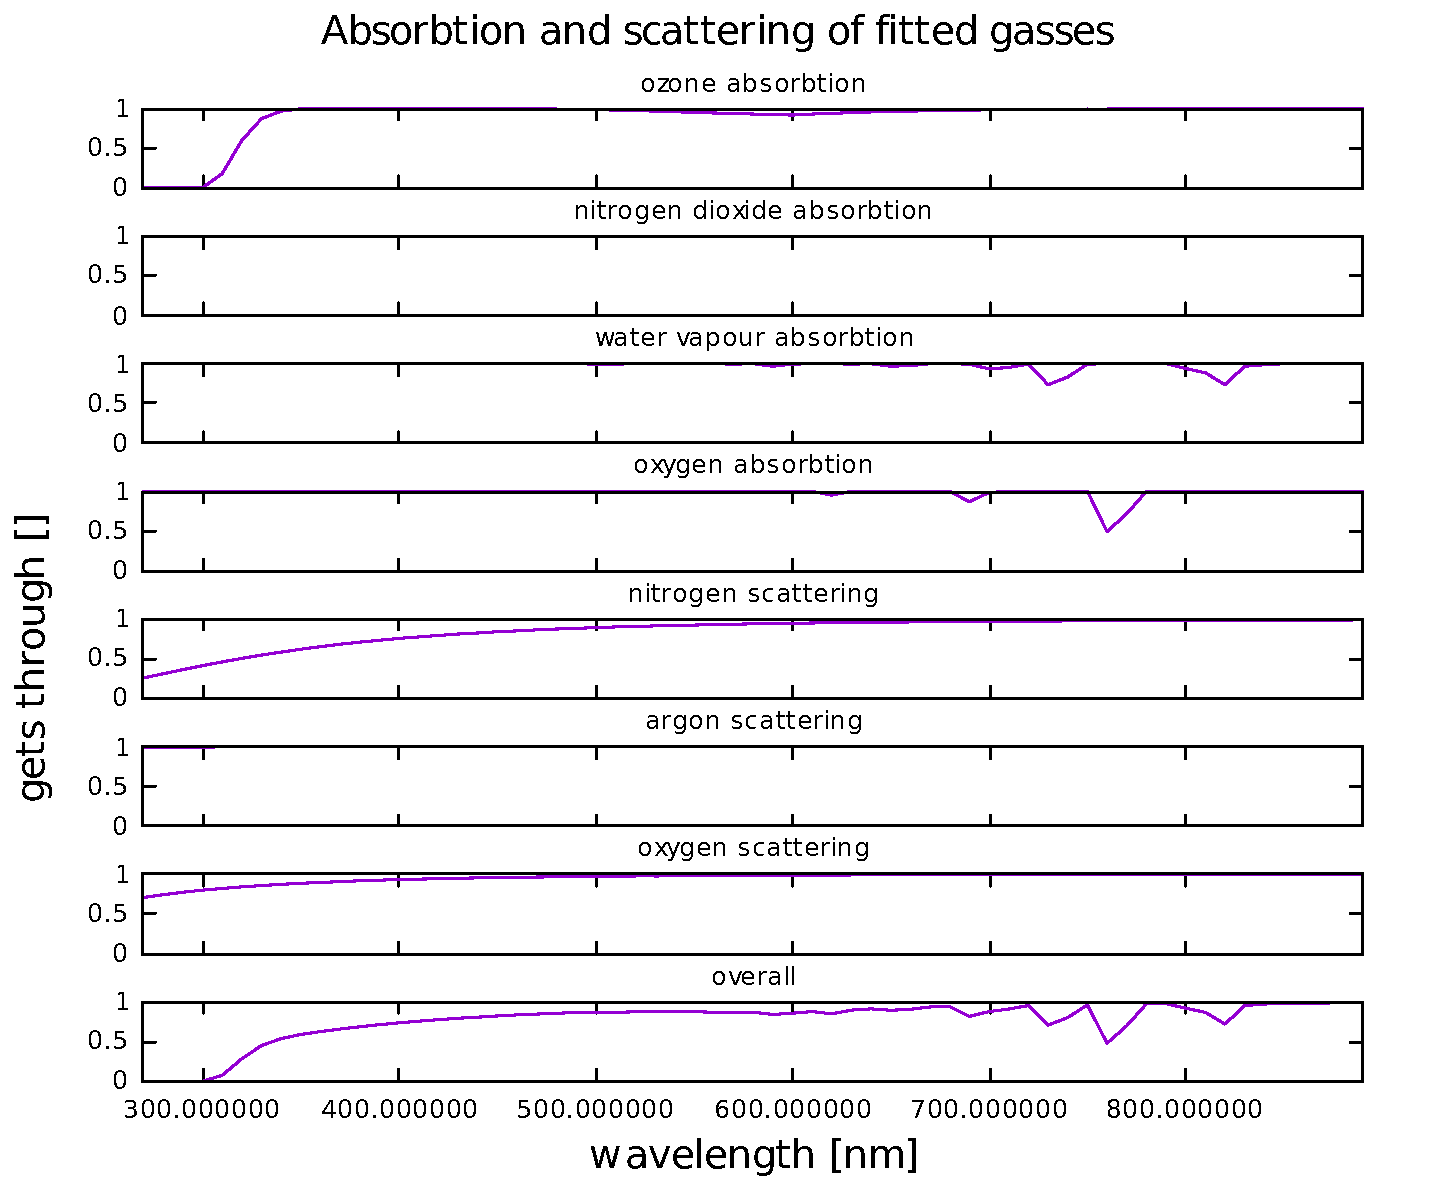
\includegraphics[width=500pt]{spectroabs.pdf}
\end{figure}
\newpage
\pagebreak
\clearpage
\section{Apendix 2}
\begin{figure}[!h]
\caption{Sensitivity curves of different sensors}
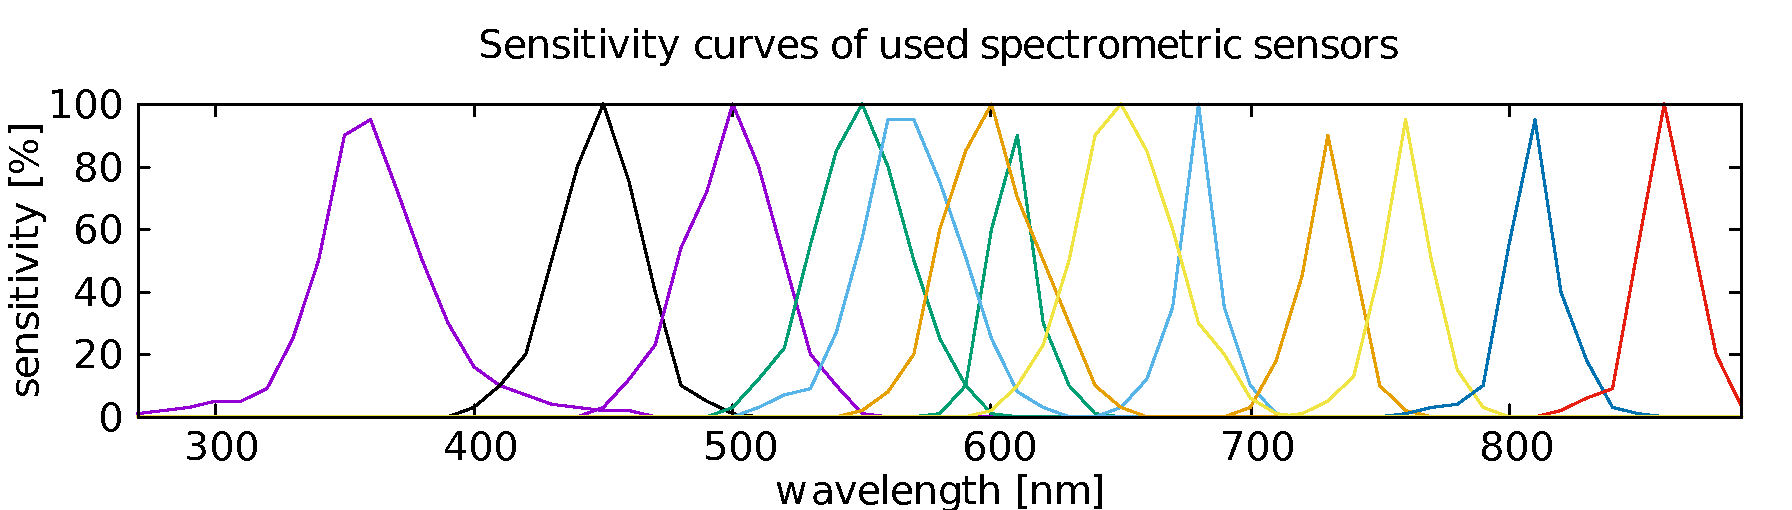
\includegraphics[width=500pt]{spectrosen.pdf}
\end{figure}

\end{document}